%!TEX root = ../thesis.tex
%*******************************************************************************
%****************************** Second Chapter *********************************
%*******************************************************************************

\chapter{\ont{} sequencing for \mtb{} public health applications: transmission clustering}

\ifpdf
    \graphicspath{{Chapter2/Figs/Raster/}{Chapter2/Figs/PDF/}{Chapter2/Figs/}}
\else
    \graphicspath{{Chapter2/Figs/Vector/}{Chapter2/Figs/}}
\fi


%%%%%%%%%%%%%%%%%%%%%%%%%%%%%%%%%%%%%%%%%%%%%%%%%%%%%%%%%%%%%%%%%%%%%%%%%%%%%%%%%
%%%%%%%%%%%%%%%%%%%%%%%%%%%%%%%%%%%%%%%%%%%%%%%%%%%%%%%%%%%%%%%%%%%%%%%%%%%%%%%%%

\section*{Publication and collaboration acknowledgements}

%=========================================================================

\section{Introduction}

%=========================================================================

\section{Dataset}


The data used for the work in this chapter and chapter 3\todo{link to chapter 3} are patient-derived \mtb{} WGS from culture. We gathered samples from Madagascar (118), South Africa (83), and England's National Mycobacteria Reference Service in Birmingham (46); giving us a total of 247 samples.  
Each sample was sequenced on both \ont{} and Illumina platforms. Our aim was to perform all sequencing for a sample from a single DNA extraction. This would ensure that any variation identified between technologies for the same sample would be due to differences in the sequencing platform and not *in vitro* evolution.  
As these samples are not reference isolates, and we want to be able to compare both Illumina and Nanopore to a "truth", we also sequenced 35 of the Malagasy isolates with PacBio.

\subsubsection{Illumina sequencing}

\towrite[inline]{need to get this information from all three collaborators}

\subsubsection{\ont{} sequencing and pre-processing}

\towrite[inline]{need to get this information from all three collaborators}

All \ont{} data for this project was basecalled and de-multiplexed using the \ont{} proprietary software tool \guppy{} (v3.4.5). We used default parameters for basecalling and the only non-default parameter used for de-multiplexing was the option to trim barcodes from the resulting sequences.  

\subsubsection{PacBio sequencing}
\unsure[inline]{is this too much detail}
35 of the Malagasy samples were sequenced and processed at the Next Generation Genomics Core within Cold Spring Harbor Laboratory. Samples were quantified with a Qubit dsDNA HS Assay Kit and QC’d through a Pulsed Field Gel Electrophoresis system. Then, samples were sheared at 10kb using a Megaruptor device and size-selected to 8-10 kb with a Blue pippin instrument - followed by 0.45X ampure bead purification. The PacBio library protocol SMRTbell Express Template Prep Kit 2.0 was used for each sample. Briefly, the first step was the removal of single-stranded overhangs followed by DNA Damage Repair, End-Repair/A-tailing, Ligation of overhang barcoded adaptors and sample pooling. A total of 3 pools were produced: LID50532 (16 samples), LID50533 (10 samples), and LID50534 (9 samples). After pooling, 0.5X ampure bead clean up was performed. A Sequel I instrument was used to sequence the 3 library pools. Libraries were annealed for an hour and bounded for an hour using sequel binding kit 3.0. Bound SMRTbell complexes were then purified with ampure beads. The run was set up as 10kb length for 10 hours movie time. The Sequel 1M V2 SMRT cells were used for each library.  
The circular consensus was called via the SMRTlink graphical user interface version 6.0.0.47841.

%=========================================================================

\section{High-quality genome assemblies for validating variant calls}
\label{sec:asm_results}

Samples with greater than 30x coverage across all three sequencing technologies were chosen to produce high-quality assemblies. In total, this left us with 9 Malagasy samples. We compare five assemblers and select the best for each sample. The reason for this comparison is that different assembly algorithms can produce quite varied results depending on sequencing technology used, species, or computational resource availability(CITE).  
The assembly tools used are Canu, Flye, Unicycler, HASLR, and Spades(CITE \& VERSION). HASLR and Unicycler are hybrid assemblers that take Illumina reads along with one long-read file, although Unicycler does not require both. Spades is also a hybrid assembler but takes an arbitrary number of different sequencing technologies. Canu and Flye are both long-read-only assemblers.

The entire assembly pipeline was orchestrated using the workflow management system Snakemake(CITE). An overview of the entire pipeline is shown in (FIGURE). The first step is trimming of adapter sequences in the Illumina reads using Trimmomatic(CITE). Two assemblies were then produced for each sample - one for each long-read technology. The exception to this was Spades, for which there is just one assembly for each sample, as it accepts all reads simultaneously. Canu, in some cases, produces assembly bubbles, which are regions where it believes there is a heterozygous locus due to differences in haplotypes. While it is not impossible some samples could be multi-clonal, we chose to remove bubbles from the Canu assemblies, effectively choosing the dominant haplotype for downstream analysis.  
All contigs in the resulting assemblies were species-classified using Centrifuge(CITE). We remove any contigs whose classification places them outside of the Mycobacterium Tuberculosis Complex.  
Polishing of the decontaminated assemblies is done in two steps. First using long reads and Racon(CITE) with default settings, followed by short reads with Pilon(CITE). Default Pilon settings were used for \ont{} assemblies, but for \pb{} we don't correct for SNPs . \pb{} CCS reads are already a consensus from multiple reads, so allowing Illumina reads to fix at a per-base level leads to decreased per-base accuracy (results not shown CITE?).  
For both polished and unpolished assemblies, we annotate using Prokka(CITE). We assess relative correctness of all assembly variations for a given sample using Assembly Likelihood Estimator (ALE)(CITE). Assembly statistics were generated for each sample using Quast(CITE) with H37Rv as a reference. We do not expect our assemblies to be the same as H37Rv, but it can provide insights into the structural completeness and genome size. Lastly, we assess per-base accuracy using a custom script. As input for the script, we provide a BAM file of the Illumina reads mapped to the assembly and the pileup generated by the Samtools subroutine \vrb{mpileup}(CITE). We provide a quorum of 90, which is the percentage of reads that must agree with the assembly at each position, and a minimum depth of 10x. Any position within the assembly that does not meet both of these conditions is considered a disagreement. The output from the script is a collection of statistics and a BED(CITE) file containing all disagreement positions.

A central component of the work in this chapter is having a way of validating the quality of variant calls, without being biased by assuming short reads are the "truth". In addition to the matched sequencing on both the \ont{} and Illumina platforms, XXX of the Malagasy samples were also sent for PacBio Circular Consensus Sequencing (CCS)\improvement{clarify this from the methods Sara sent - i.e. is HiFi more correct?}. CCS produces so called HiFi reads, which have a base-level accuracy greater than 99.9\%(CITE). The reason these reads have such a high accuracy is that each one is the consensus from multiple passes of the DNA enzyme around a circular copy of the original double-stranded read. As the HiFi reads are both long and accurate, they are now being regularly used to produce high quality \denovo{} assemblies and complete existing reference genomes(CITE).  

Due to the lack of extensive benchmarking of assembly methods for CCS, and \mtb{} more generally, we undertook to determine what combination of technologies and methods would give us the best "truth" genomes. There has been comprehensive analysis of \ont{} and hybrid assemblies for \ecoli{}(CITE), but its genomic characteristics are very different to those of \mtb{}. For this analysis we chose to assess five assemblers: \vrb{flye}, \vrb{canu}, \vrb{spades}, \vrb{unicycler}, and \vrb{HASLR}(CITE). Both \vrb{unicycler} and \vrb{HASLR} are hybrid assemblers, which means they utilise both long and short reads. We use them to produce Illumina/CCS and Illumina/\ont{} assemblies. The only tool capable of operating with all three technologies (at the time of writing) is \vrb{spades}. One assembly for each long read technology was produced with \vrb{canu} and \vrb{flye}.  
Each assembly was additionally polished with their relevant long reads and Illumina data using \vrb{racon} and \vrb{pilon} respectively. These combinations resulted in 18 assemblies (9 polished and 9 unpolished) for assessment.  

Assessing the quality of \denovo{} assemblies is non-trivial and requires aggregation of various metrics(CITE). Whilst a reference genome exists for \mtb{}, there are enough differences between the lineages that using this reference would not be appropriate for our purposes. We will look at each assessment metric individually, and then decide on the best assembly method from this information

\subsubsection{Assembly Likelihood Evaluation score}

The assembly likelihood evaluation (ALE) score is a reference-free metric that describes the likelihood of an assembly given it's \kmer{} distribution, and the likelihood of the reads being generated from that assembly. It combines information such as read quality, agreement in the alignment of reads to assembly, mate-pair orientation, paired-end read length, and depth of sequencing. Importantly, the ALE score can be used to compare assemblies of the same genome, which is exactly the use case we have. Whilst ALE scores and not insightful on their own, the difference \textit{between} assembly scores gives the relative probability of correctness. So for each sample, we are interesting in the assembly that has the \textit{highest} ALE score.  

Across the 9 samples, \vrb{flye} has the highest ALE score in five cases, whilst \vrb{spades} was the most probable assembly in two, with \vrb{unicycler} and \vrb{canu} having the maximum score in one sample each (\autoref{fig:ale_score}). Note, this is considering both polished and unpolished assemblies together for each tool. When considering which long read sequencing technology produces the greatest ALE score, CCS had the top score in 7/9 samples. In 6/9 samples, the highest ALE score was from a polished assembly.\unsure{is this figure necessary or are the numbers in the text sufficient?}



\begin{figure}
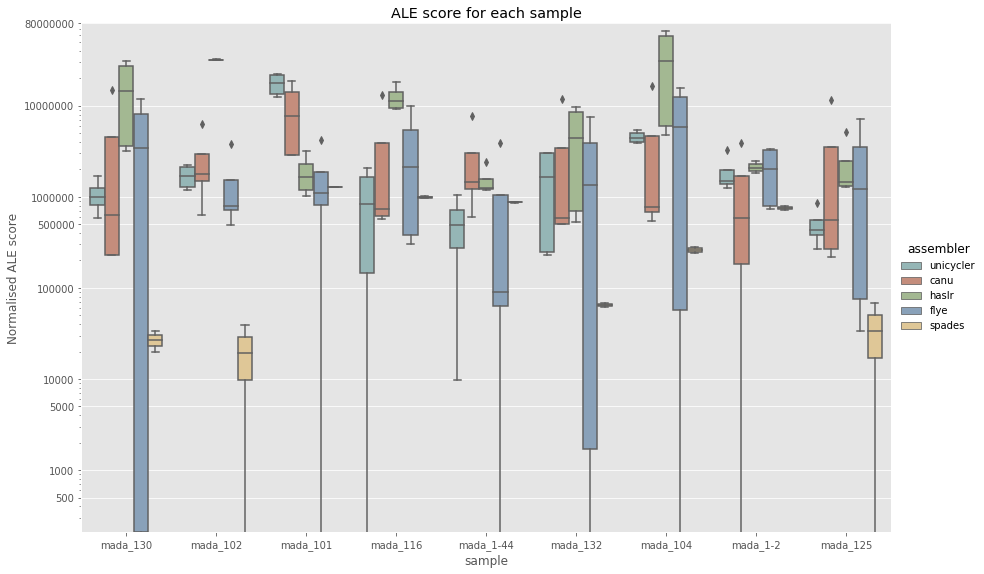
\includegraphics[width=1.0\textwidth]{Chapter2/Figs/ale_score.png}
\centering
\caption{The normalised ALE score (Y-axis) for each sample (X-axis), coloured by assembly tools. ALE score is a metric describing the likelihood of an assembly. The normalisation is done by subtracting the assembly's score from the maximum (best) score for that sample, giving a relative probability of correctness. Each box represents different technologies and polishing status for each assembler.}
\label{fig:ale_score}
\end{figure}



\subsubsection{Disagreement rate}

The disagreement rate is an approximation of the per-base accuracy of the assembly (see Methods\todo{link to relevant methods section}). In short, we map Illumina reads to the assembly and calculate what proportion of positions do XXX\% of the reads agree with the assembly nucleotide.  

In 7/9 samples, a \vrb{HASLR} assembly had the lowest disagreement rate, followed by \vrb{unicycler} having the minimum in 2/9. Polished genomes produced the lowest disagreement rate in 8/9 samples and \ont{}-based assemblies had the best accuracy in 6/9 samples. While it isn't so surprising that assemblies polished with Illumina reads have a lower disagreement rate, it is unexpected that \ont{} would produce more accurate assemblies (\autoref{fig:disagree_rate}). One caveat to keep in mind here - and this is the reason for looking at many different metrics - is that there is an element of overfitting to this metric: we assess using Illumina, and so naturally, assemblies polished with Illumina produce better results. That is not to say this statistic is void, but that it should be used with caution.



\begin{figure}
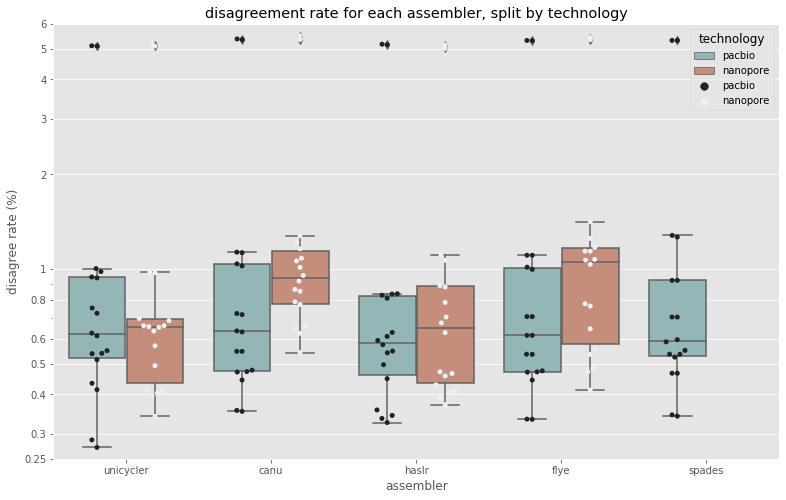
\includegraphics[width=1.0\textwidth]{Chapter2/Figs/disagree_rate.png}
\centering
\caption{The disagreement rate (Y-axis) for each assembler (X-axis), coloured by the sequencing technology. Disagreement rate is the percentage of sites in the assembly where Illumina reads do not have XX\% quorum. Each box/point represents different samples and polished status for the relevant assembler-technology combination.}
\label{fig:disagree_rate}
\end{figure}



\subsubsection{Number of contigs}

As \mtb{} has only a single, circular chromosome, for an assembly to be structurally complete, there should only be a single contig in the final assembly. However, it is not always appropriate for an assembly method to produce a single contig as data quality, depth of sequencing, read length, and/or repetitive content of the genome can hamper this goal(CITE). Conversely, receiving a single contig as output is no guarantee of it's quality for similar reasons to the previous, multi-contig scenario. For the purposes of this benchmark, considering on conjunction with the other metrics, the number of contigs can be a useful datum for selecting our favoured assembly. If an assembly has a single contig, and scores well on other metrics, we would be more inclined to choose it over another assembly with similar metrics, but many more contigs.

Across all combinations of assembly conditions, \vrb{spades} (8/18), \vrb{flye} (18/32) and \vrb{canu} (16/32) produced far more single-contig assemblies than the hybrid methods (\autoref{fig:num_contigs}). \vrb{unicycler} produced no single-contig genomes, whilst \vrb{HASLR} yielded only 2/32. When considering sequencing technology, CCS (26/72) had many more single-contig assemblies than \ont{} (10/72). Note: \vrb{spades} assemblies use all three technologies and are not considered in the technology single-contig totals.



\begin{figure}
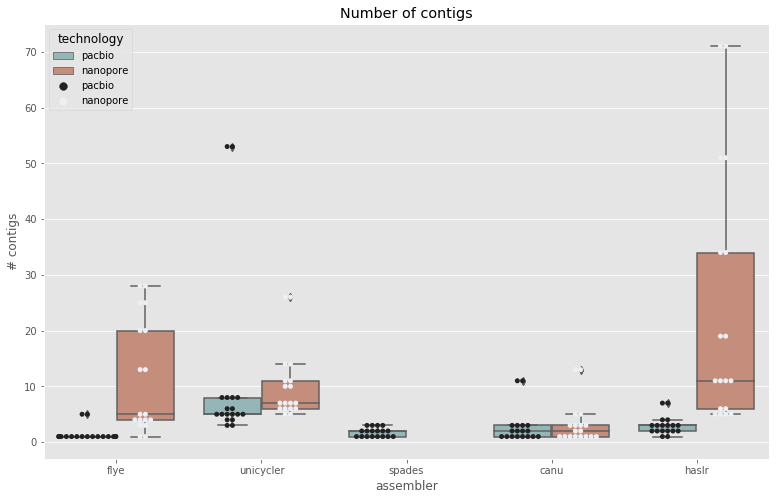
\includegraphics[width=1.0\textwidth]{Chapter2/Figs/num_contigs.png}
\centering
\caption{The number of contigs (Y-axis) produced from each assembly (X-axis), coloured by sequencing technology. Each box/point represents different samples and polished status for the relevant assembler-technology combination.}
\label{fig:num_contigs}
\end{figure}



\subsubsection{Length of assembly}

As mentioned earlier, comparing the assemblies to the \mtb{} reference genome (H37Rv; accession: `NC\_000962.3`) is not appropriate, however, it's length/size can be used as an aid for selection. The size of the any lineage's genome is not expected to differ from the reference by more than about X kilobases(CITE). Considering the genome size in addition to disagreement rate is particularly informative. It would be quite easy for an assembly method to produce very accurate per-base contigs but refusing to produce sequence for "harder" parts of the genome. While such an assembly would score well on disagreement rate, it would not do so well when considering how close to the expected genome size it is. The length of the assembly is also clearly shows when a method is outputting \textit{too much} sequence.

When comparing the size of each assembly to that of H37Rv, we found a fairly even spread across assemblers for the closest size to H37Rv. For 3/9 samples, \vrb{canu} has the smallest size difference, followed by \vrb{spades} (2/9), \vrb{unicycler} (2/9), \vrb{HASLR} (1/9) and \vrb{flye} (1/9). An honourable mention should be made of \vrb{flye} and \vrb{spades} as they had much lower variation in size compared to the other approaches. In terms of sequencing technology, in 6/9 samples CCS produced the genome size closest to H37Rv. Polished assemblies had the closer size in 5/9 samples.



\unsure[inline]{should I use the non-zoomed version of \autoref{fig:asm_len}?}
\begin{figure}
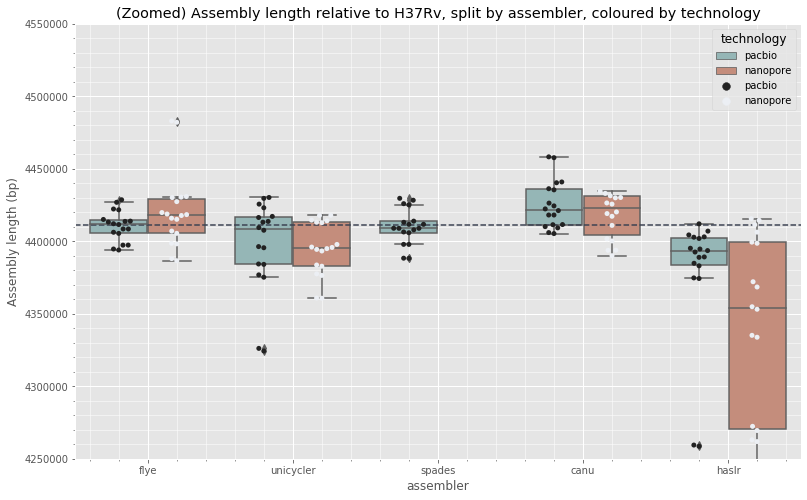
\includegraphics[width=1.0\textwidth]{Chapter2/Figs/asm_len.png}
\centering
\caption{Size/length (Y-axis) of each assembly (X-axis), coloured by each sequencing technology. The horizontal dashed line represents the size of the \mtb{} reference genome (4,411,532bp). Each box/point represents different samples and polished status for the relevant assembler-technology combination. Note: the Y-axis has been limited to allow for greater resolution of similarity to the H37Rv size}
\label{fig:asm_len}
\end{figure}



\subsubsection{Contamination detection}

The decontamination step in the assembly pipeline (\todo{reference relevant section in methods}) revealed that one sample, `mada\_1-2`, contained contigs from three different species: *Mycobacterium intracellulare*, *Dermacoccus nishinomiyaensis*, and *M. tuberculosis*. These contigs were all at sufficient coverage to not be considered background noise. For the assembly assessment analysis only the contigs from \mtb{} were used, but figures for the assessment metrics in the previous subsections show this sample is an outlier in almost all metrics. Given this profuse contamination, `mada\_1-2` will not be used in any analysis where these assemblies are used for truth validation purposes.


\unsure{should this paragraph stay here or move to the conclusion?}In conclusion, considering all assessment metrics, \vrb{flye} and \vrb{spades} assemblies were consistently the better performing methods across all of the criteria outlined in this section. As most of the validation analyses that these assemblies will be used for involve comparing Illumina and \ont{} data to a "neutral truth", the unpolished CCS assemblies from \vrb{flye} were selected for use in the remainder of this chapter. The differences between the polished and unpolished CCS assemblies was almost negligible and do not outweigh the benefit of having a single-technology PacBio assembly that can be used as an unbiased reference point for comparing the other two technologies.

%=========================================================================

\section{Quality control of samples}
\label{sec:ch2-qc}

Prior to any variant calling, all samples were subjected to a quality control (QC) pipeline to ensure all data used was of the highest quality. The QC pipeline was written in \vrb{snakemake}(CITE) and an overview of the steps can be seen in (FIGURE). \\
The first step in QC is decontamination of both Illumina and \ont{} sequencing reads. We use the decontamination database from \vrb{clockwork}(CITE), which contains a wide range of organisms, including viral, human, \mtb{}, NTM, and nasopharyngeal-associated bacterial genomes. Each genome has associated metadata indicating if it is contamination or not. Reads are mapped to the database using `bwa mem`(CITE) (Illumina) and \vrb{minimap2}(CITE). The resulting alignment is used to quantify the proportion of reads considered contamination, unmapped, and wanted. A read is considered wanted if it has any mapping to a non-contamination genome in the database and is output to a final decontaminated fastq file. All other mapped reads are considered contamination. Interactive \vrb{krona}(CITE) charts (see FIGURE\change{move the reference to the krona chart to the results section}) are used to visualise a sample's composition based on the decontamination database alignment.  

All decontaminated fastq files were subsampled to a depth of 60x (Illumina) and 150x (\ont{}) using \vrb{rasusa}(CITE). The reason for subsampling is to limit unnecessarily large read sets that can drastically slow down later steps in the analysis process and do not provide any benefit\unsure{see if there is a reference that backs this up}. Any sample with depth less than the maximum threshold remains unchanged.  

The last step in the QC pipeline is to assign lineages for each sample. A panel of lineage-defining SNPs from (CITE) is used in conjunction with a sample's VCF from the Illumina variant calls(LINK) for the lineage assignment. At each lineage-defining position in the sample's VCF we determine if the called allele is the same as the panel allele. If it is, we add the full lineage that allele defines (e.g. 4.1.1) to a list of called lineages. For this analysis, if more than one heterozygous call was made at lineage-defining positions, we abandon lineage assignment for that sample. After classifying all of a sample's lineage-defining positions we then produce a lineage assignment based on the list of called lineages. The most recent common ancestor of all the called lineages is used as the lineage assignment. For example, if the called lineages were [4, 4.2.3, 4.2.5] the lineage assignment would be 4.2. If there is more than one called lineage from a different major lineage group, a mixed lineage assignment is given. For example [4, 4.2.3, 4.2.5, 3.2] would still be called lineage 4.2, however, [4, 4.2.3, 4.2.5, 3.2, 3.1] would be called mixed.

The purpose of QC is to ensure all samples used in later analysis are of the highest quality. By highest quality we mean all samples have perfectly matched Illumina and \ont{} data, sufficient coverage on both sequencing technologies, no contamination, and no evidence of a mixed \mtb{} population. Prior to the QC stage, N samples were excluded as their Illumina and \ont{} reads were not from the exact same DNA extraction.  

After filtering out unmapped/contaminant reads and subsampling all samples to 60x (Illumina) and 150x (\ont{}), N samples were excluded from further analysis due to low coverage (FIGURE) - defined as Nx for Illumina and Nx for \ont{}. An example chart of the composition of genomes from the decontamination database for a sample can be seen in (FIGURE).  

Lastly, N samples were excluded as their lineage assignment was either called mixed or unknown. Unknown lineage assignments can happen if the sample has too many heterozygous calls as lineage-defining positions, or there was no called lineages at any lineage-defining position.  

In the end, we have N samples that have passed QC and will be used for the remainder of this chapter.

\towrite[inline]{Make sure to mention the samples excluded as their Illumina and ONT data do not match based on the discrepancy in variant calls}


%=========================================================================

\section{Construction of \mtb{} reference graphs}
\label{sec:tbprg}

% https://github.com/mbhall88/head_to_head_pipeline/issues/10 and https://github.com/mbhall88/head_to_head_pipeline/issues/9 have some good plots/stats to include here
\pandora{} requires a \prg{} in order to operate. For the work in this chapter, we chose to construct a reference \prg{} based on the \mtb{} reference genome, H37Rv. We add variants sampled from 15000 global \mtb{} isolates gathered by the \cryptic{} consortium\improvement{confirm this number and see if there is a reference for the samples}. We sampled at two different rates to evaluate how varying complexity of \prg{}s affect variant-calling precision and recall.

To ensure the reference \prg{} is not biased towards a particular lineage we first split the global \cryptic{} VCF into separate lineage VCFs. Lineages were determined for each of the global samples using the same approach as in \autoref{sec:ch2-qc}. Lineages 1-4 were separated into separate VCF files and all other lineages were grouped into a single VCF due to much smaller representation. Variants calls from 14 high-quality \mtb{} assemblies, representing lineages 1-7, were also included in this "other" lineage VCF. The two \prg{} complexities we chose to construct were termed "sparse" and "dense". From each lineage VCF, we took a random subsample of 50 and 200 samples and combined them into single sparse and dense VCFs respectively. It should be noted that we use the same fixed random seed for the subsampling to ensure the sparse \prg{} is a subset - with respect to the sample variants - of the dense \prg{}. We filtered the resulting VCFs to remove any positions with no alternate allele calls, or that failed the filtering applied by the \cryptic{} pipeline (except for masked positions).  

The \prg{} that \pandora{} uses as it's reference is actually a collection of local \prg{}s (loci). These loci are effectively partitions of the original genome; one can partition based on any criteria they like. For the work in the chapter, we chose to split the H37Rv genome based on the genomic features outlined in the accompanying General Feature Format (GFF). We also retain the segments *between* the features - so called intergenic regions (IGRs). We combine genomic features that have overlapping coordinates (i.e. they are transcribed on opposite strands or different reading frames) into a single locus and also join any locus (feature or IGR) shorter than 500bp with its 3' neighbour. By building the reference \prg{} in this manner we ensure that every position in the H37Rv genome is represented in one of the local \prg{}s. We then remove any locus with 30\% or more of its positions overlapping a genome mask of repetitive regions in H37Rv \cite{tbmask2014}. Refer to \autoref{app:mask} for a detailed description of why this masking strategy was chosen.

We form the sparse and dense \prg{}s by applying the variants from their VCF to the template sequence of each locus for the corresponding genomic position. For each position in the VCF, we infer the locus it corresponds to. We then take all (called) alternate alleles and create a sequence for each; that is, the template sequence, with the reference allele starting at the position replaced with the alternate allele. Note, we disregard any indels longer than 20bp or that span a locus boundary. All of these sequences are pooled into a single fasta file for each locus. 

The multi-sequence fasta files are then subjected to multiple sequence alignment (MSA) using MAFFT(CITE). We use the accurate global alignment setting, G-INS-i(CITE\info{citation in Papers library under msa tag}), with default parameters, using the \vrb{ginsi} script provided with MAFFT. The resulting MSA is then converted to a \pandora{}-compatible \prg{} using the `make\_prg` script(CITE) with a maximum nesting level of 5 and maximum match length of 7. All of the local \prg{}s are then combined into a single \prg{} file and indexed with \pandora{} using a \kmer{} size of 15 and window size of 14. In the end, we have two single \prg{} files - sparse and dense.

\subsection{Computational performance}

An important consideration for usability of any genomic method is the computational costs such as time and resources. The construction process just outlined need only be run once and then it can be used as a reference for subsequent \pandora{} usage. However, it is important to understand the time and resources required in order to identify bottlenecks. Additionally, if the resource usage is high enough, it may also limit who is able to build their own reference graph. We outline the time and memory requirements for each step of the graph construction in \autoref{tab:build-prg}. All times are on a single compute node with 32 CPU cores. We only report the MSA, \makeprg{}, and \pandora{} index steps as these are constants that must be done this way and the steps prior to this are not very time or resource intensive and could be done in a number of different ways.

\begin{table}
\centering
\begin{tabular}{|l|l|l|l|l|l|l|}
\hline
         & \multicolumn{3}{l|}{Sparse}                          & \multicolumn{3}{l|}{Dense}                           \\ \hline
Step     & CPU time (sec) & Wall clock (H:m) & Max. memory (Gb) & CPU time (sec) & Wall clock (H:m) & Max. memory (Gb) \\ \cline{1-2} \cline{4-5} \cline{7-7} 
MSA      & 138576         & 1:16             & 209              & 445284         & 3:56             & 301              \\ \cline{1-2} \cline{4-5} \cline{7-7} 
Make PRG & 3746           & 0:04             & 0.9              & 4269           & 0:05             & 0.9              \\ \cline{1-2} \cline{4-5} \cline{7-7} 
Index    & 142            & 0:01             & 1.5              & 361            & 0:01             & 1.7              \\ \cline{1-2} \cline{4-5} \cline{7-7} 
\end{tabular}
\caption{Computational time and memory usage for the main steps of building a \mtb{} reference graph. Sparse and Dense refer to two different densities with respect to the number of variants used. All steps were run on a single compute node with 32 CPU cores. MSA=multiple sequence alignment;PRG=population reference graph.}
\label{tab:build-prg}
\end{table}

%=========================================================================

\section{Calibration of \ont{} variant filters}

Filtering of variant calls is integral to creating trusted transmission
inference. There are many such filters used for Illumina genomic data
and they can produce inconsistent results\cite{walter2020}. Before
attempting to define SNP thresholds for Nanopore data, we explore the
performance of a range of filtering parameters for both bcftools and \pandora{}.  
The aim of this filter calibration is ultimately to determine if SNP-calling precision for \ont{} is comparable with Illumina, and if not, how close can we get it.
We evaluate the resulting, filtered SNP calls
against the COMPASS\todo{http://dx.doi.org/10.2807/1560-7917.es.2019.24.50.1900130} Illumina SNP calls for the seven
samples with high-quality PacBio assemblies (see Section \autoref{sec:asm_results}) to ensure no bias for
Illumina or Nanopore.
For others interested in investigating variant filters for \ont{} data, we also hope this calibration acts as a good starting point for deeper analysis.

\subsection{Validating variant calls}

We evaluate the precision and recall of the SNP calls using the method outlined in \todo{link to varifier stuff in chapter 1} - \vrb{varifier} - with a flank length of 100bp. The samples we evaluated are those seven with PacBio assemblies (see Section \autoref{sec:asm_results}). As a truth genome for each, we use the unpolished \vrb{flye} PacBio assembly, along with a mask for low-quality regions. These low-quality regions were identified by aligning the sample's Illumina reads to the assembly with \vrb{bwa mem} and flagging any position with less than 10 reads mapping to it or less than 90\% agreement. From the varifier output, we use the edit distance measure for both precision and recall. All results were visualised in Python using the matplotlib (version 3.1.3) (Hunter 2007) and seaborn (version 0.11.1) (Waskom 2020) libraries.

\subsection{Illumina variant calling}

Illumina variant calls were made using the COMPASS pipeline (Jajou 2019) used by Public Health England (PHE). Briefly, reads are mapped to the \mtb{} reference genome, and \vrb{samtools mpileup} is used to identify SNPs (Li 2009). SNPs are filtered based on the following criteria: i) must have at least five high-quality supporting reads, ii) must have at least one read in each direction, iii) 75\% of reads must be high-quality, iv) the diploid genotype must be homozygous, v) fraction of reads supporting the major allele must be at least 90\%. In addition, any SNPs falling within masked sites - as defined by aligning the \mtb{} reference to itself and identifying repetitive regions - are excluded.

\subsection{\ont{} variant calling: \vrb{bcftools}}
\label{sec:bcftools-filters}

As there is no standard variant caller used for \mtb{} \ont{} data, we chose to try bcftools, as it has a long history of use in bioinformatics, is one of the main variant callers used for Illumina data  and is readily available to all users, and is much more user-friendly than other available tools. Another main reason for its use is that it is the updated form of the samtools pipeline used by COMPASS. The parameters used are
relevant to the variant calls produced by the multiallelic
model\todo{http://dx.doi.org/10.1099/mgen.0.000418}.

Nanopore reads were aligned to the \mtb{} reference genome using minimap2 (version 2.17), with options to produce SAM output containing no secondary alignments. The subsequent SAM file is provided as input to the bcftools (version 1.11) subcommand \vrb{mpileup} with the 'skip indels' option. The resulting pileup is then used to call SNPs with \vrb{bcftools call} using the multiallelic caller with a haploid model and an option to skip indel variants.
There are a number of fields in the resulting VCF relating to the information about the reads that support each position. We filter VCF positions based on whether certain fields meet a given criteria.
After a thorough examination of the how filtering based on each field impacts precision and recall, we settled on five filters for bcftools. First, we filter out positions with a quality (QUAL field) score of less than 60. The quality is a log-scaled probability for the assertion made by the alternate allele. Second, read position bias (RPB) of at least 0.05 is required. RPB indicates whether there is a bias for support from the ends of reads, as they are usually low quality. Third, we filter out positions with a segregation-based metric (SGB) less than -0.5. SGB is a measure of how read depths across alleles match expected depths. Fourth, variant distance bias (VDB) less than 0.002 is filtered out. VDB is a measure of whether a variant's position within the reads that support it is randomly distributed or biased (e.g. near the start). Fifth, the fraction of reads supporting the called allele (FRS) must be 90\% or more.



\autoref{fig:bcftools-filters} shows the precision (proportion
of calls that are correct) and recall (proportion of variants found) for
a selection of these bcftools VCF fields. The trade-off between
precision and recall is dependent on the question one is trying to
answer. For the purposes of transmission clustering, we place higher importance on
precision as we seek to ensure the calls used are of the highest
quality. The consequence of this is we miss some variants - compared to
COMPASS.

The filtering we use for the remainder of the transmission inference
work is to remove any VCF record (variant) with a quality score (QUAL)
of less than 60,~ a read position bias (RPB) of less than 0.05, variant
distance bias (VDB) less than 0.002, a fraction of read-support (FRS)
less than 0.9, and a segregation-based metric (SGB)~ greater than -0.5.
These filters, represented by the yellow box in
Figure~{\ref{fig:bcftools-filters}}, lead to median precision and
recall of 99.94\% and 84.26\%, respectively for the seven validation
samples. When compared to the COMPASS median precision and recall values
of 100\% and 92.58\%, respectively,~ we produce Nanopore variant calls
with equivalent precision to Illumina, but with less recall.



\begin{figure}
\begin{center}
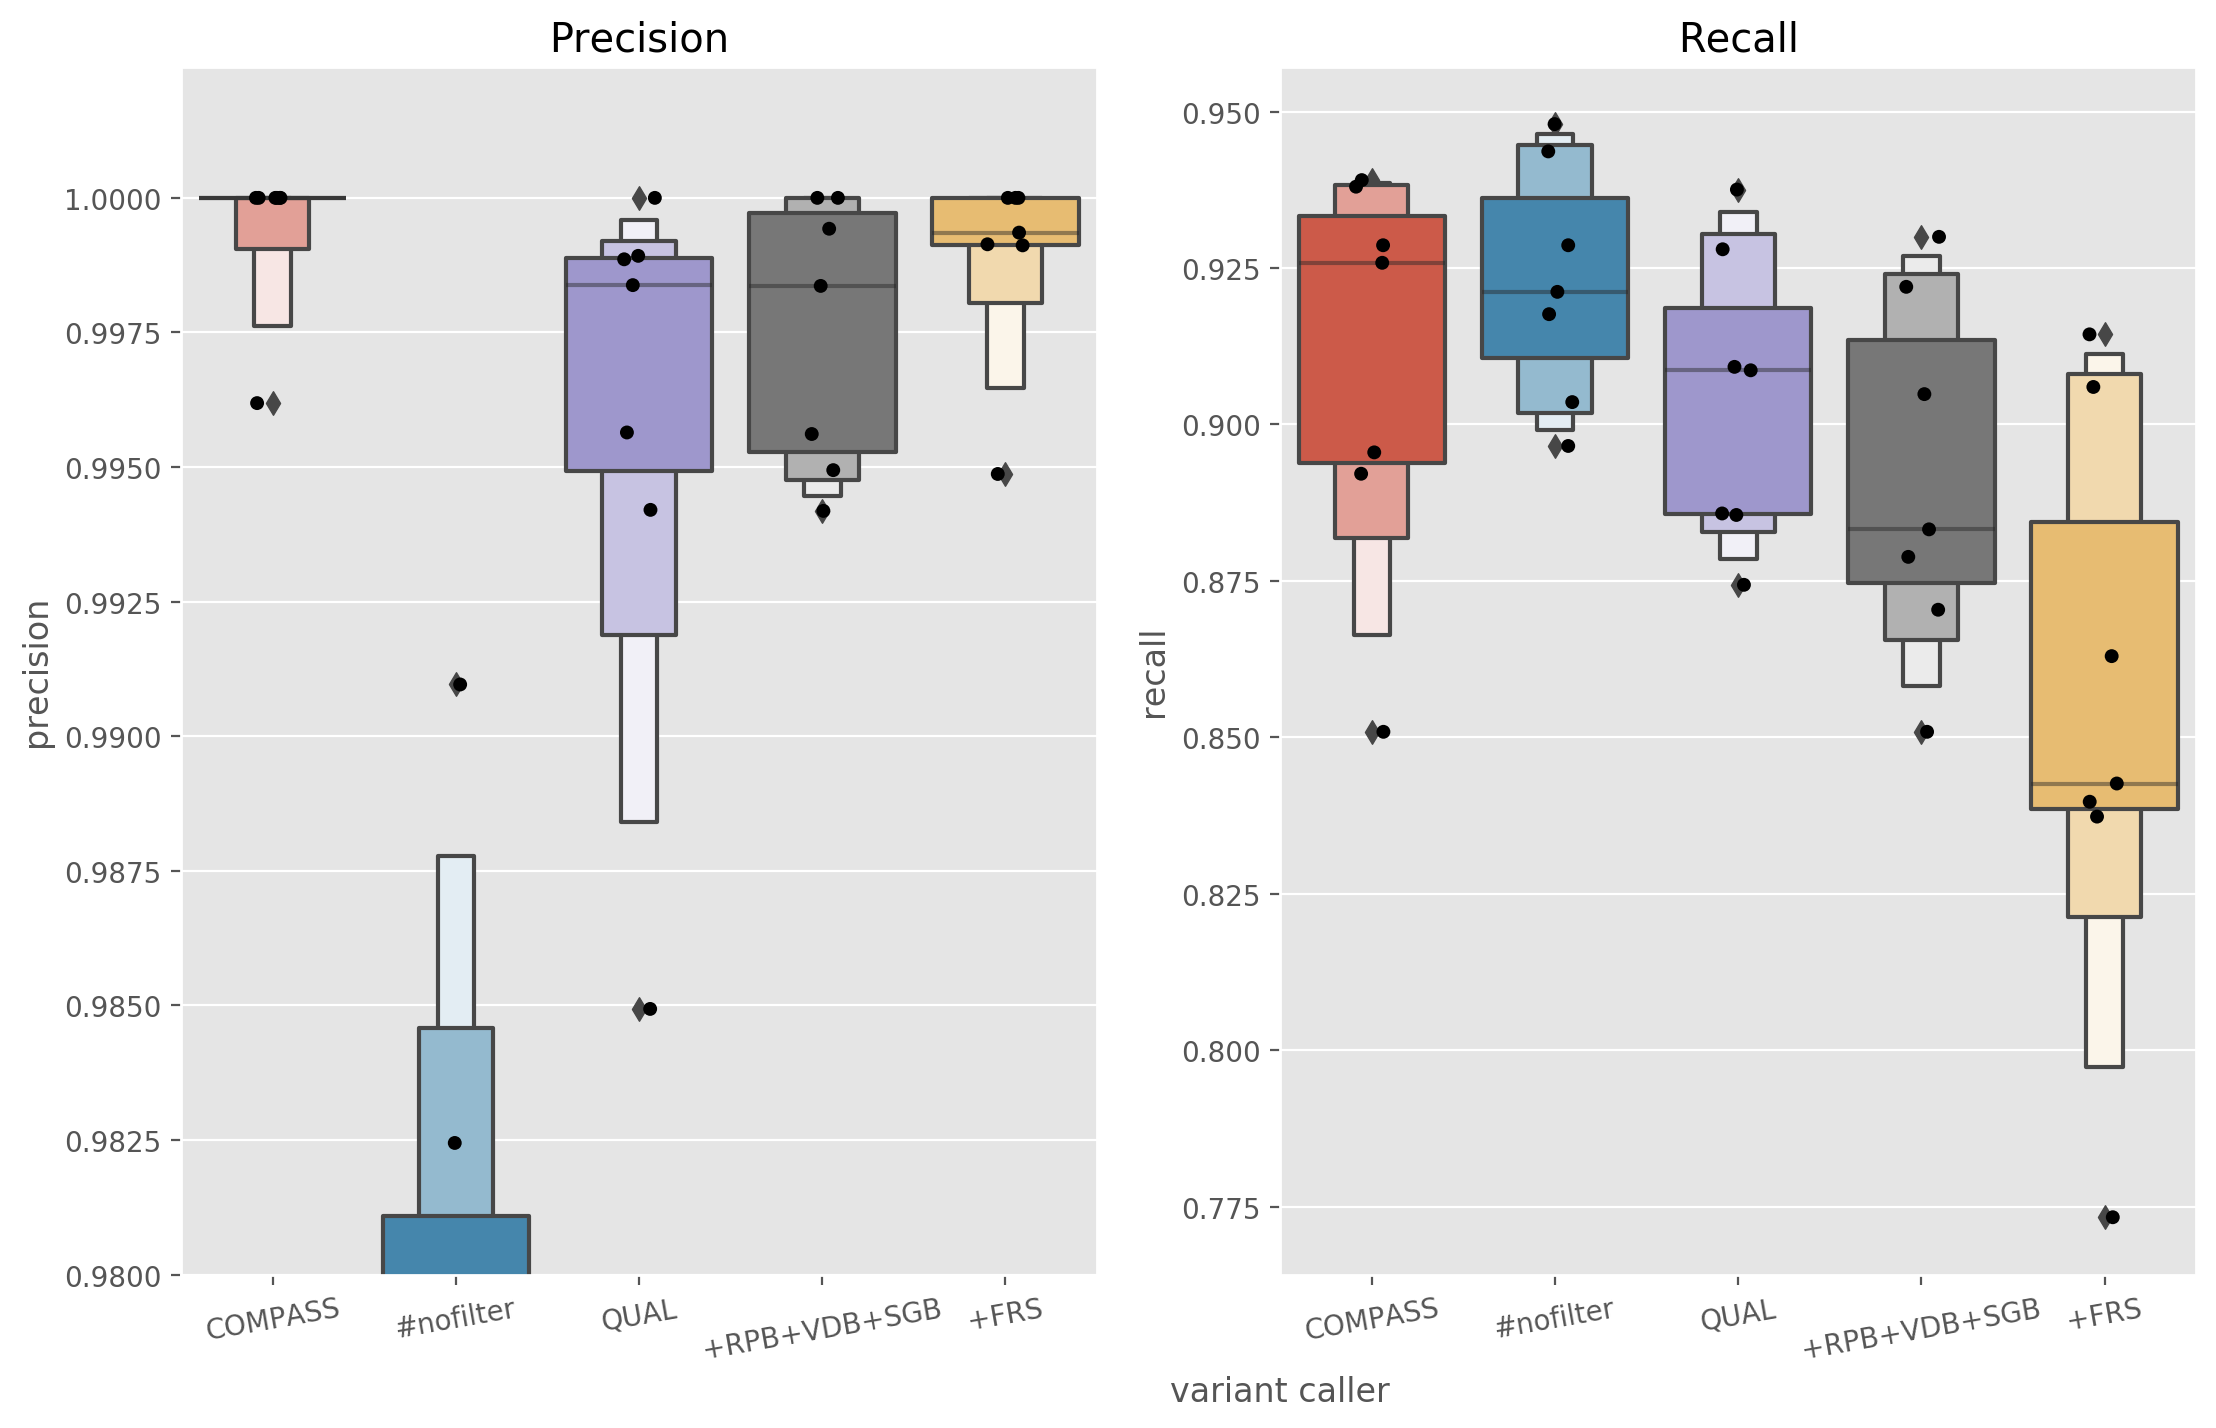
\includegraphics[width=0.70\columnwidth]{Chapter2/Figs/bcftools-precision-recall-filters.png}
\caption{{Precision (left) and recall (right) of SNPs for COMPASS (red) and a
selection of bcftools filters. `\#nofilter' (blue) is bcftools with no
filtering of variants. `QUAL' (purple) is bcftools SNPs with a quality score of
60 or more. `+RPB+VDB+SGB' (grey) indicates bcftools variants with the INFO
field values~\(\ge\)0.05,~\(\ge\)0.002,
and~\(\le\)-0.5, respectively, plus QUAL. `+FRS' (yellow) shows
bcftools SNPs with all previous filters, plus only SNPs where the
fraction of reads supporting the variant is at least 90\%. Note: the
precision plot y-axis was cut causing some `\#nofilter' points to be
hidden.
{\label{fig:bcftools-filters}}%
}}
\end{center}
\end{figure}


\subsection{\ont{} variant calling: \pandora{}}
\label{sec:pandora-filters}

When assessing the best filters for increasing the precision of variant calls from \pandora{}, we are also interested in determining whether \prg{} density has a noticeable impact on performance. We use the sparse and dense \prg{}s from \autoref{sec:tbprg} and look at precision and recall these produce for the same filters.
For each sample, we discover \denovo{} variants using the method outlined in \autoref{chap:denovo} using the \vrb{discover} command of \pandora{} (version 0.8.0), using default parameters except for limiting the number of novel variants for a candidate region to 10. Novel variants are added to the relevant \prg{} using the same method as \todo{reference chapter 1 section that outlines how we feed de novo variants back into the PRG} and the resulting, update \prg{}s are indexed with \pandora{}. The \vrb{map} routine of \pandora{} is then used to genotype the sample's reads and produce a VCF. To be able to compare the \pandora{} VCF to the truth assemblies we tell \pandora{} to output coordinates with respect to the H37Rv reference sequence for each locus. Then, we convert these locus positions to the absolute position within H37Rv. Running \pandora{} in this way leads to some alleles being quite long and having a lot of redundant information, so we use bcftools norm to trim unused alleles and reduce variants down to their most succinct representation.
The \pandora{} VCF fields we use for filtering are: the depth of coverage on the called allele, which we require at least 3 reads; we keep positions with a strand bias of at least 1\%, which is the lowest depth on the forward or reverse strand divided by the total depth; a genotype confidence score no less than 5; an FRS of at least 90\%  - calculated the same way as in \autoref{sec:bcftools-filters}.
The results of incrementally applying these filters, along with no filters and COMPASS, are shown in \autoref{fig:pandora-filters-snps}. \pandora{}'s best median precision (100\%) and
is with a sparse \prg{} and all filters applied. With all filters, the sparse \prg{} leads to a median recall of 71.99\%. When compared to the COMPASS median precision and recall values
of 100\% and 92.58\%, respectively, \pandora{} produces Nanopore variant calls
with equivalent precision to Illumina, but with 20.59\% less recall. Despite this large difference in recall, we chose to use all of the filters outlined above because, as mentioned earlier, precision is far more important than recall for the transmission cluster work.
In nearly every filtering combination, the sparse \prg{} lead to higher recall \emph{and} precision. As a result, the remaining work featuring \pandora{} in this chapter will use the sparse \prg{}.


\begin{figure}
\begin{center}
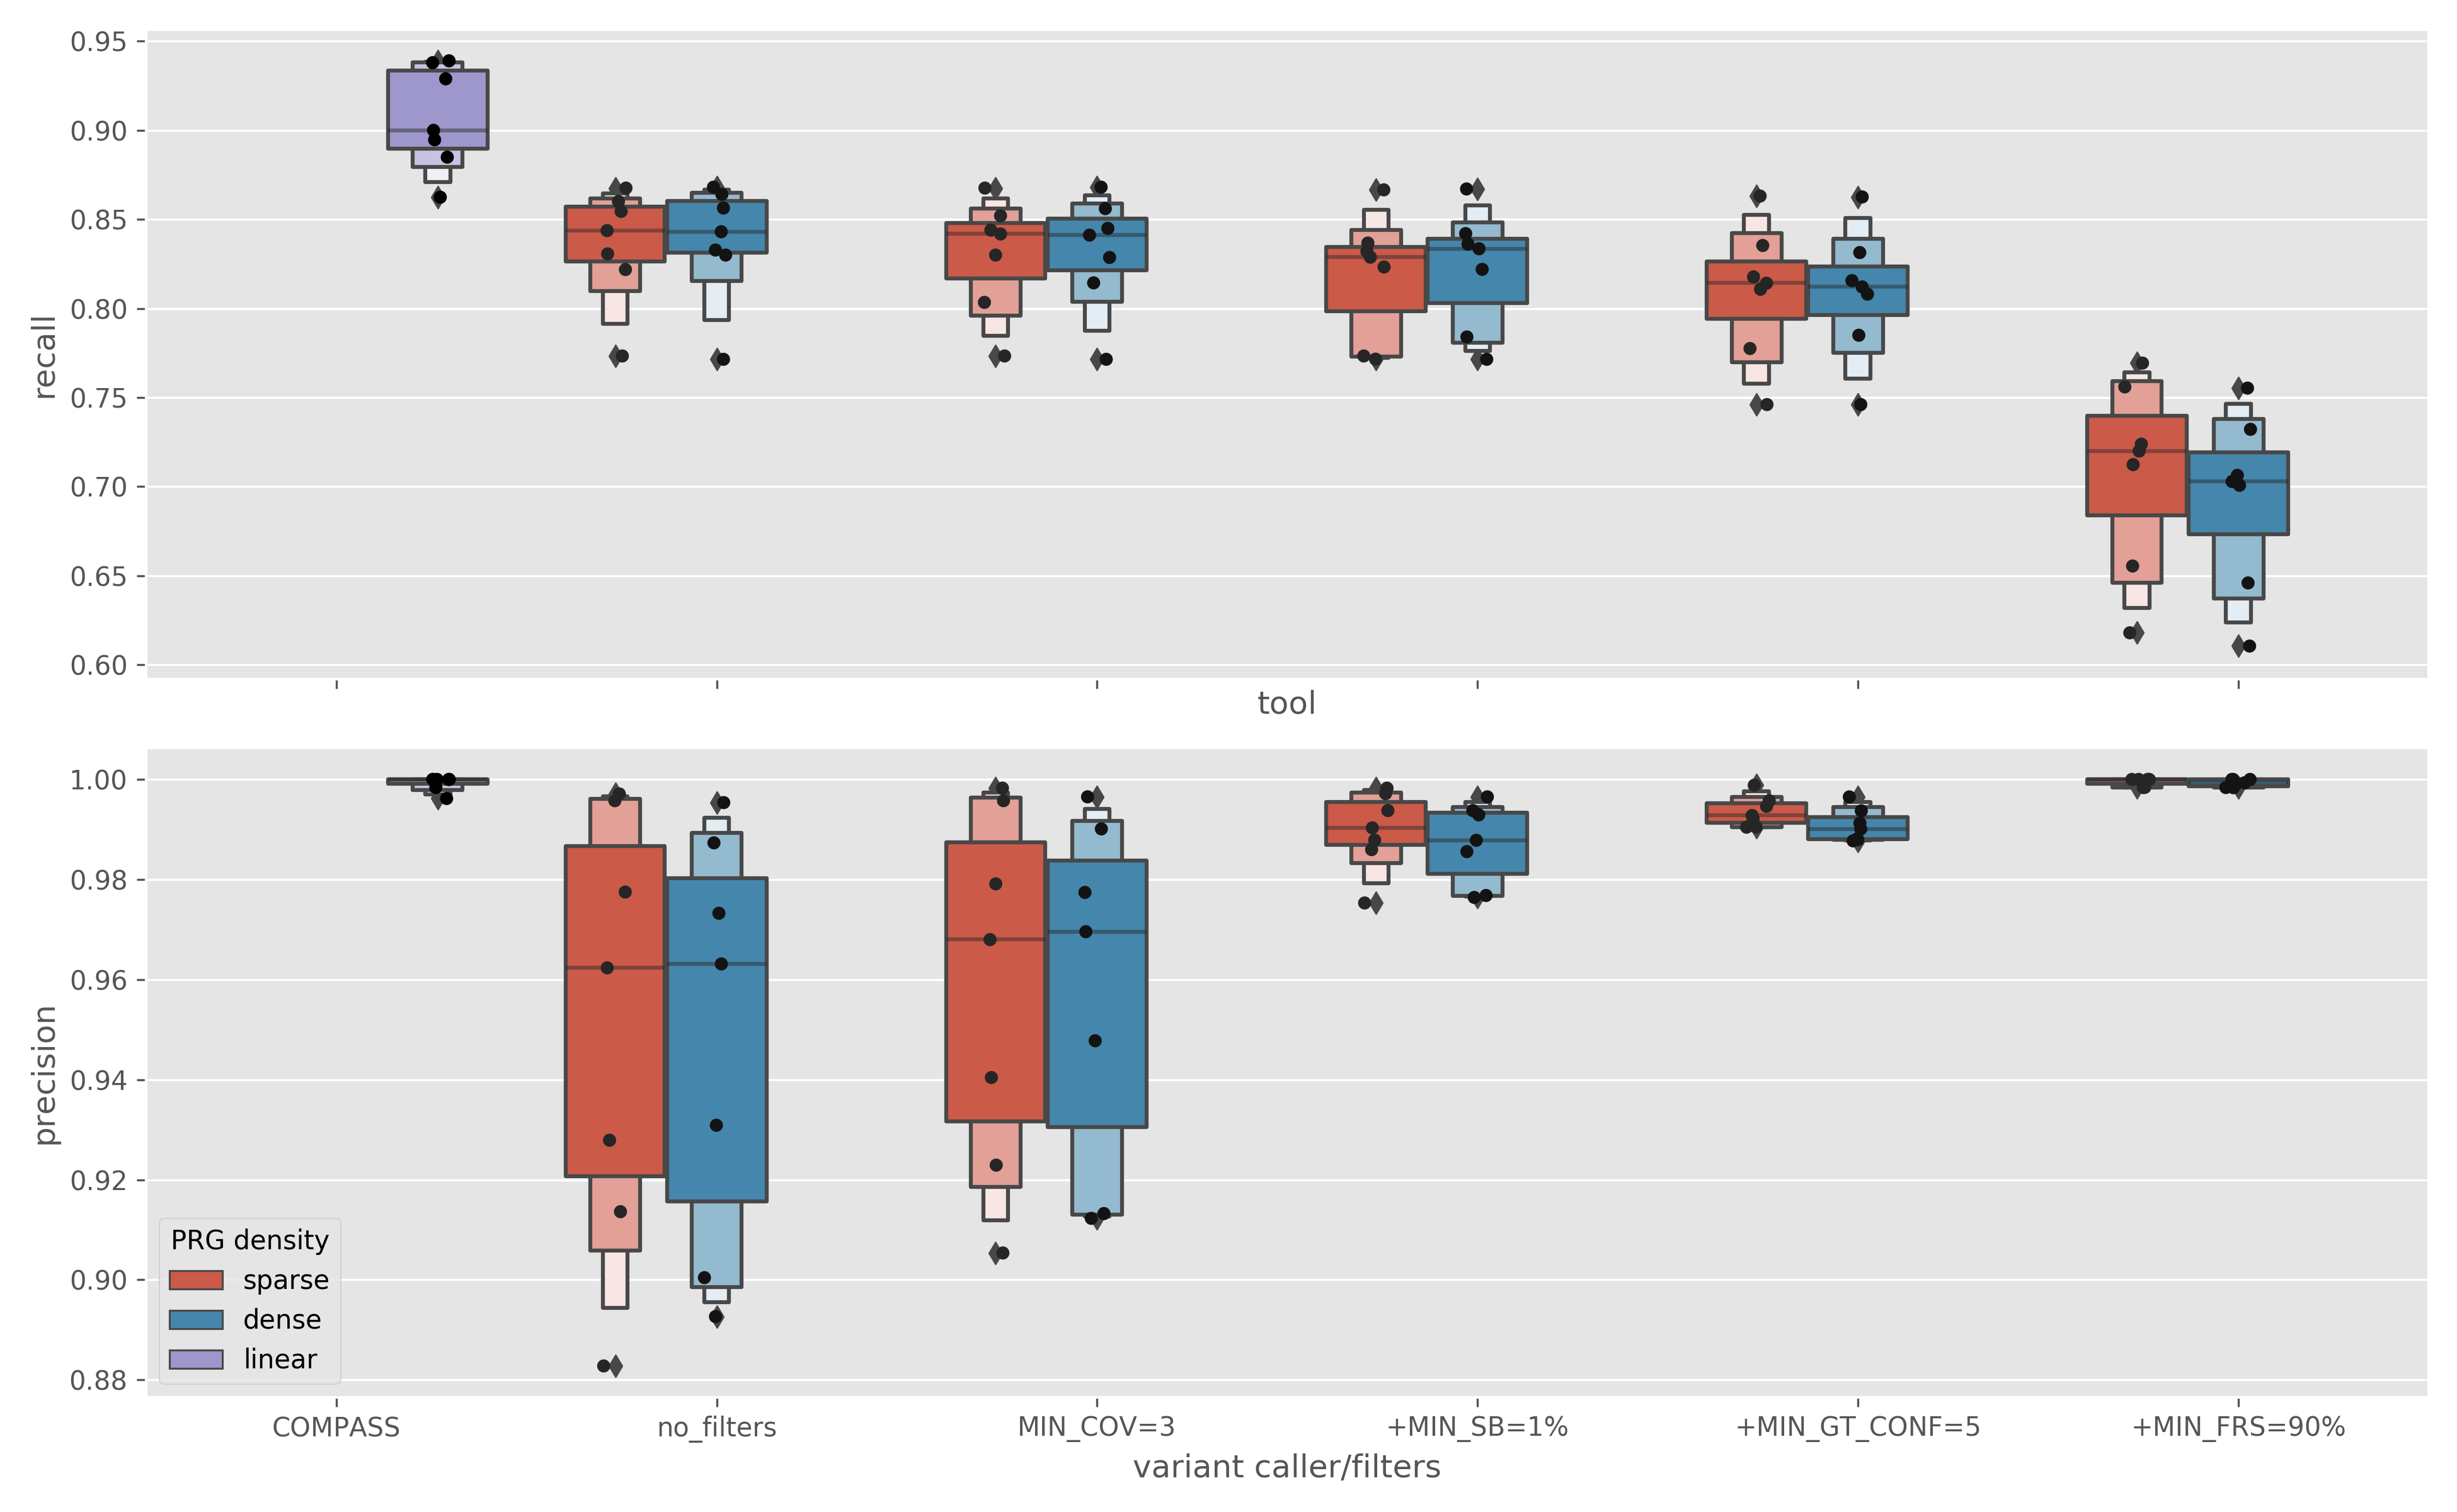
\includegraphics[width=0.70\columnwidth]{Chapter2/Figs/pandora-precision-recall-filters-snps.png}
\caption{{Precision (bottom) and recall (top) of SNPs for COMPASS (purple) and \pandora{} with sparse (red) and dense (blue) \prg{}s. The \pandora{} boxes start with no filters on the left, with each box moving to the right adding a filter to the previous box. The COMPASS box is a reference to the precision and recall of Illumina variant calls. Linear PRG density refers to the fact that COMPASS uses a single, linear reference genome as opposed to \pandora{}, which uses a genome graph. The black points refer to single data points for the seven samples used. MIN\_COV=minimum depth of coverage;MIN\_SB=minimum strand bias;MIN\_GT\_CONF=minimum genotype confidence score;MIN\_FRS=minimum fraction of read support.
{\label{fig:pandora-filters-snps}}%
}}
\end{center}
\end{figure}


Although we only use SNPs for identifying transmission clusters, we also assessed \pandora{} variant calls for all variants, including indels up to a length of 20bp in \autoref{fig:pandora-filters-all}.  We did this for the sake of future work that might be interested in using \pandora{} indel calls, such as predicting drug resistance. Again, the sparse \prg{} gave better precision and recall than the dense one. Using all variants, there was a recall improvement to 75.48\% (all filters) - up 3.49\% from SNPs only. Precision on the other hand sees a drop to 95.90\% when assessing all variants - compared to 100\% for SNPs only.

\begin{figure}
\begin{center}
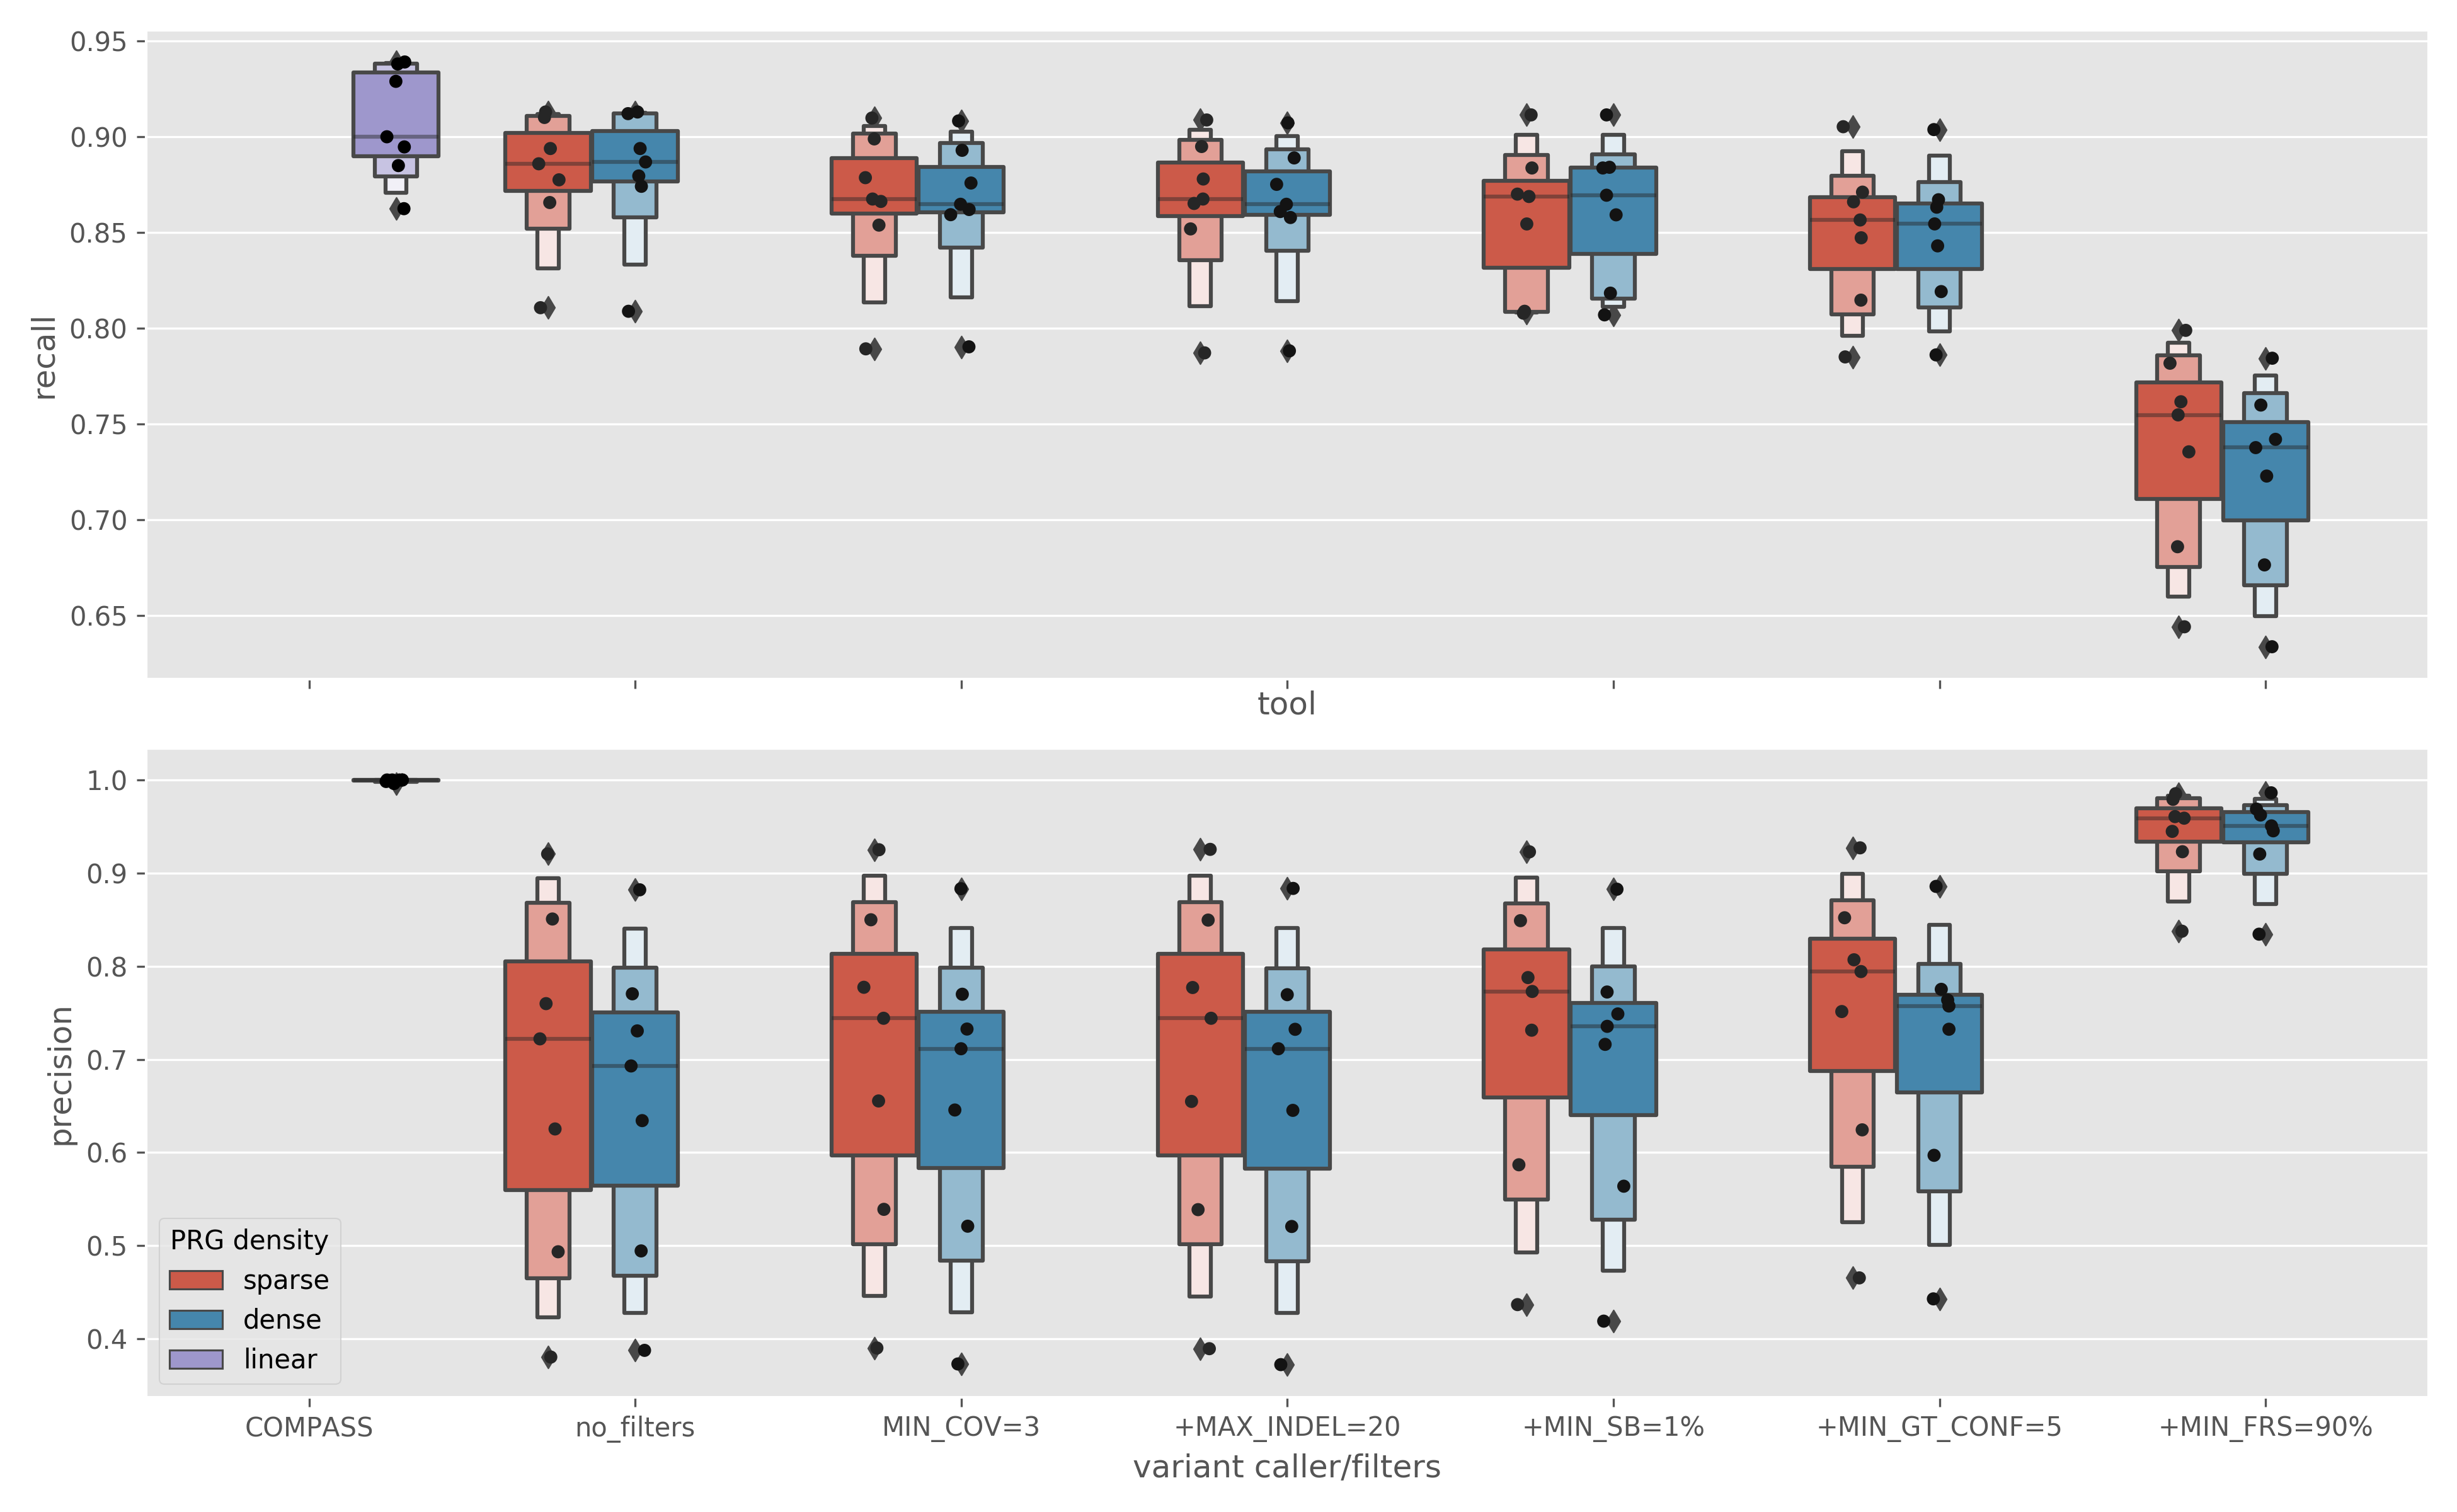
\includegraphics[width=0.70\columnwidth]{Chapter2/Figs/pandora-precision-recall-filters-all-variants.png}
\caption{{Precision (bottom) and recall (top) of SNPs for COMPASS (purple) and all variants (maximum indel length of 20bp) for \pandora{} with sparse (red) and dense (blue) \prg{}s. The \pandora{} boxes start with no filters on the left, with each box moving to the right adding a filter to the previous box. The COMPASS box is a reference to the precision and recall of Illumina variant calls. Linear PRG density refers to the fact that COMPASS uses a single, linear reference genome as opposed to \pandora{}, which uses a genome graph. The black points refer to single data points for the seven samples used. MIN\_COV=minimum depth of coverage;MIN\_SB=minimum strand bias;MIN\_GT\_CONF=minimum genotype confidence score;MIN\_FRS=minimum fraction of read support.
{\label{fig:pandora-filters-all}}%
}}
\end{center}
\end{figure}

\towrite[inline]{talk about all variants results}

%=========================================================================

\section{Pairwise SNP distance comparison for Illumina and \ont{} sequencing data}

To determine the distance between samples, we first generate sample consensus sequences for both sequencing modalities. This consensus sequence is obtained by applying the calls from a given VCF to the Mtb reference genome. We nullify (mark as 'N') any positions were i) the position failed filtering, ii) the reference genome position does not appear in the VCF file, iii) the genotype is null, or iv) the position is within the reference mask (see section 2.4). All consensus sequences for a sequencing technology are joined into a single FASTA file and a pairwise distance matrix is calculated using snp-dists (Seemann 2018).
Figure 3 was created in Python using the matplotlib and seaborn libraries. All pairwise comparisons between a sample and itself were removed from the visualisation, and only a single value was used for each pair (i.e. we keep sample1 vs. sample2 and discard sample2 vs. sample1 as they are the same). RANSAC Robust Linear Regression (Fischler 1981), as implemented in the Python library scikit-learn (Pedregosa 2011), was used for determining a linear equation and line-of-best fit for the relationship between pairwise Illumina and Nanopore SNP distance.

When attempting to infer transmission clusters, the accepted approach is
to define a SNP distance threshold and say that any genomes within this
distance of each other are clustered. It follows that the SNPs used must
be trusted. Having shown that precision on par with Illumina can be
achieved with Nanopore data, we investigate the pairwise SNP distance
between samples produced by both sequencing technologies. The intention
here is to determine whether the thresholds typically used for Illumina
data can also be used for Nanopore, or whether adjustments need to be
made.

The pairwise SNP distance relationship can be seen in
Figure~{\ref{638875}}. For a given pair of samples, we
plot their SNP distance, based on the COMPASS (Illumina) variant calls,
against the SNP distance for the same pair, based on the bcftools
(Nanopore) variant calls. If the same thresholds used for Illumina can
also be used for Nanopore, we would expect the distances to be the same
and the bulk of the points in the plot to fall on the dashed, diagonal
identity line. What we see instead is a linear relationship that falls
slightly~\emph{under} this identity line. Given the filtered Nanopore
SNP calls made by bcftools have a recall XX\% lower than Illumina, this
is expected, as we miss some SNPs found by Illumina.

One important observation though is highlighted by the zoomed inset in
Figure~{\ref{638875}}. As SNP thresholds used for Mtb
are generally well below 100, it makes more sense to base SNP distance
relationships on those samples that are ``close''. And indeed, when we
zoom in on pairs of samples within 100 (Illumina) SNPs of each other, we
see an association that falls closer to the identity line. Fitting a
linear model to this close subset of pairwise distances, yields a
relationship defined by the equation~\(y=0.808x+0.559\).
Replacing~\(x\) with an Illumina SNP threshold gives the
(predicted) equivalent Nanopore SNP threshold based on this
relationship.~ For example, at an Illumina SNP threshold of 12, the
linear equation would predict a corresponding Nanopore SNP distance of
10.~



\begin{figure}
\begin{center}
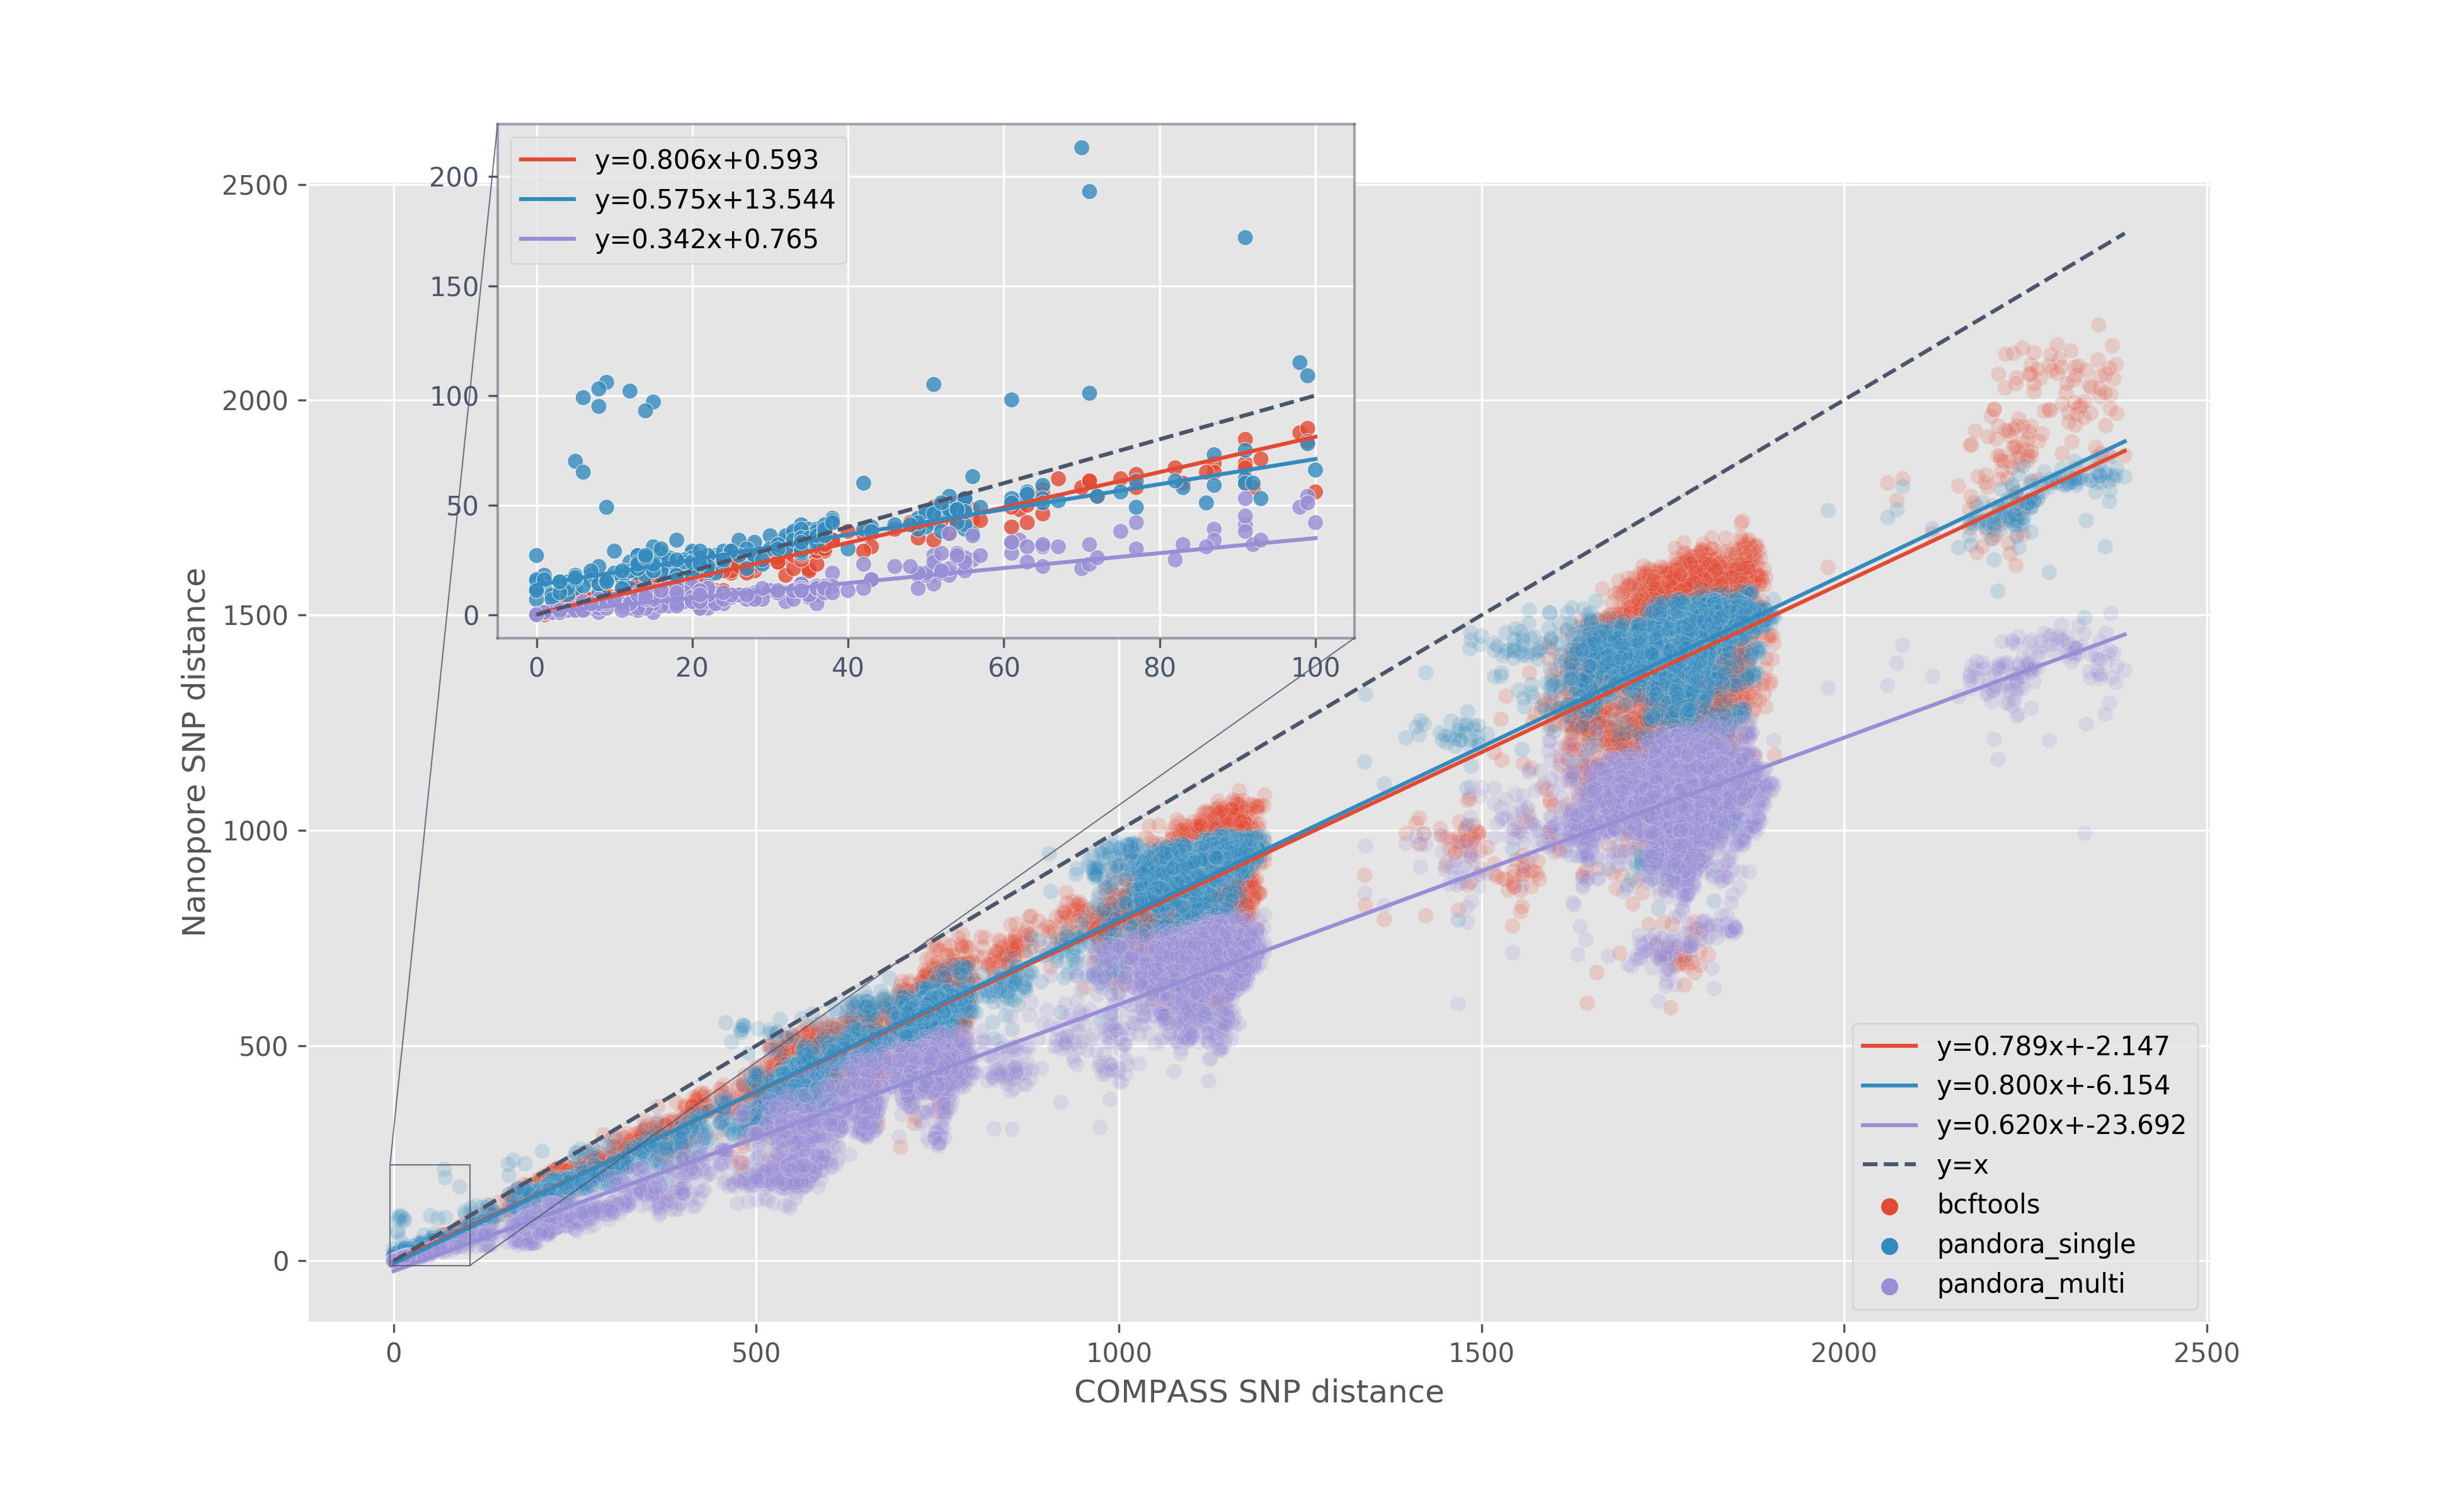
\includegraphics[width=0.70\columnwidth]{Chapter2/Figs/combined-dotplots.png}
\caption{{Pairwise SNP distance relationship between Illumina (COMPASS; x-axis)
and Nanopore (bcftools; y-axis) data. Each point represents the SNP
distance between two samples. The black, dashed line shows the identity
line (i.e. y=x) and the blue line shows the line of best fit based on
the robust linear model fit to the data. The zoomed inset shows all
pairs where the COMPASS distance is~\(\le100\).
{\label{638875}}%
}}
\end{center}
\end{figure}



%=========================================================================

\section{SNP threshold-based \ont{} transmission clustering}

Selecting a SNP threshold to infer transmission clusters from has seen a
variety of values recommended\todo{http://dx.doi.org/10.1093/molbev/msy242}. As we seek to show
concordance of Nanopore data with PHE's Illumina-based strategy, we opt
for threshold values 0, 2, 5, and 12. PHE define two cases as clustered
if they have a SNP distance $\le$ 12 as "\emph{although 12
SNPs represents the maximum SNP difference between 2 isolates for which
epidemiological links have previously been identified
\todo{http://dx.doi.org/10.1016/s1473-3099(12)70277-3} and is a conservative measure for reporting
isolate relatedness}"~\todo{https://www.gov.uk/government/publications/tuberculosis-in-england-annual-report}. Five was likewise selected as
it was found by~\todo{http://dx.doi.org/10.1016/s1473-3099(12)70277-3} to indicate membership in a recent
transmission chain. Threshold values 0 and 2 were chosen to provide
insight into the level of granularity possible and is of clinical
interest in certain settings (personal correspondence).



In order to cluster samples, for a given SNP threshold $t$, we use only pairs of samples in the distance matrix with a distance $\le t$ to define a graph, $G=(N,E)$, where samples ($N$) are connected by weighted edges ($E$), with the weight of an edge indicating the distance between the two samples it connects. Clusters are defined as the set of connected components $\{C_1, C_2...C_N\}\in G$, where $N$ is the number of clusters. That is, a cluster (connected component), $C_i$, is a subgraph of $G$ where a path exists between any two samples in $C_i$, but no path exists to any samples in the rest of $G$. With this definition, all clusters have a minimum of two members. \\
To assess how closely Nanopore SNP-based clustering approximates Illumina SNP-based clustering we use a similarity measure on sets, the Tversky Index \todo{http://dx.doi.org/10.1037/0033-295x.84.4.327}. We define the Illumina clustering as $G$ and the Nanopore clustering as $H$ and formulate the Tversky Index as $$TI=\frac{\sum_{n}^{N_G}\frac{\left|C_{n,G}\cap C_{n,H}\right|}{\left|C_{n,G}\cap C_{n,H}\right|+\alpha |C_{n,G}-C_{n,H}|+\beta |C_{n,H}-C_{n,G}|}}{|N_G|}$$
where $N_G$ is the set of samples (nodes) in $G$ and $C_{n,G}$ is the cluster in $G$ that sample $n$ is a member of. When $\alpha = 1$ and $\beta=0$ we get the Sample-Averaged Cluster Recall (SACR) and when $\alpha = 0$ and $\beta = 1$ we get the Sample-Averaged Cluster Precision (SACP). SACR states, on average, what proportion of the samples clustered together in $G$ are also clustered together in $H$ - it is a measure of how many true positives Nanopore retains. Likewise, SACP states, on average, what proportion of the samples clustered together in $H$ are also clustered together in $G$ - it is a measure of how many extra samples Nanopore adds to clusters. \\
SACR and SACP do not inherently account for when $H$ has clusters containing no samples in $G$. In order to quantify any extra clustering by $H$, we characterise the Excess Clustering Rate (XCR) as the proportion of singletons (unconnected nodes) in $G$ that are (incorrectly) connected in $H$. We define this as
$$XCR = \frac{|A-B|}{|A|}$$
where $A$ is the set of singletons in $G$ and $B$ is the set of singletons in $H$.



\emph{{Note about the above paragraph}}

We implement SACR, SACP and XCR calculation in Python with
the~\texttt{networkx} library~\todo{Aric A. Hagberg, Daniel A. Schult, Pieter J. Swart. Exploring Network Structure, Dynamics, and Function using NetworkX. 11 - 15 In Proceedings of the 7th Python in Science Conference. (2008)}. For a given threshold,
we create the Illumina clustering (graph),~\(G\), and the
Nanopore clustering,~\(H\). For each sample (node)
in~\(G\), we count the number of samples in it's cluster
(neighbours) in both~\(G\) and~\(H\). To
determine SACR we divide the number of neighbours by the number of
samples in it's cluster in~\(G\). Likewise, we determine
SACP by dividing the number of neighbours by the number of samples in
the sample's cluster in~\(H\). Both SACR and SACP are the
mean for all samples in~\(G\). Suppl. Figure X illustrates
this process.

Figure~{\ref{827243}} is a visualisation of these
clustering results. The graphs represented are~\(G\) - one
for each SNP threshold. The inner and outer parts of each node
represents the SACR and SACP values, respectively, for the cluster it is
a member of.~

\subsection{Linear reference approach}

It is one thing to look at the relationship between Illumina and
Nanopore pairwise SNP distance, but ultimately the most important
question is: do Nanopore SNPs lead to transmission clusters consistent
with those obtained with Illumina SNPs? To answer this question, we
compare Illumina- and Nanopore-based clusters for{ four
clinically-interesting (Illumina) SNP thresholds -} 0, 2, 5, and 12. For
the clustering of the Nanopore data, we use the same SNP threshold as
Illumina, except for 12 - we use 11 for Nanopore instead.

Transmission clusters are generated by connecting two node when the
distance between them is less than or equal to the SNP threshold. The
connected components (nodes) in the resulting graph are the transmission
clusters. We produce such graphs for Illumina and Nanopore pairwise
distances and for all four SNP thresholds.

To assess whether Nanopore transmission clusters are consistent with
their Illumina counterparts, we define two evaluation metrics:
Sample-Averaged Cluster Recall (SACR) and Precision (SACP). Full
definitions for SACR and SACP can be found in {[}link to methods{]}.
Briefly, for each sample in an Illumina-defined cluster, SACR is the
proportion of samples in it's Illumina cluster are also in it's Nanopore
cluster - averaged over all samples. SACP is the proportion of samples
in it's Nanopore cluster are also in it's Illumina cluster - averaged
over all samples. SACR indicates whether samples have been missed from
Nanopore clustering (false negatives) and SACP reveals if additional
samples are being added to Nanopore clusters (false positives). One
shortcoming of SACR and SACP is they do not account for when the
Nanopore clustering contains clusters where no member of the cluster is
part of an Illumina cluster. To that end, we also define Excess
Clustering Rate (XCR) as the proportion of Illumina non-clustered
(singleton) samples that are clustered by Nanopore. A value of 0.1 would
indicate that 10\% of non-clustered samples were actually part of a
cluster in the Nanopore clustering.

Figure~{\ref{827243}} shows the results running the
above evaluation. For all four SNP thresholds analysed, Nanopore
achieves a SACR of 1.0 - meaning Nanopore does not miss any samples from
clustering. For Illumina SNP thresholds 0, 2, 5, and 12, Nanopore
produces SACP values of 1.0, 0.966, 0.949, and 0.845 respectively. In
addition, the XCR values obtained are 0.015 (2/137 singletons), 0.008
(1/128), 0.057 (7/122), and 0.031 (3/97) for the respective SNP
thresholds.~


\begin{figure}
\begin{center}
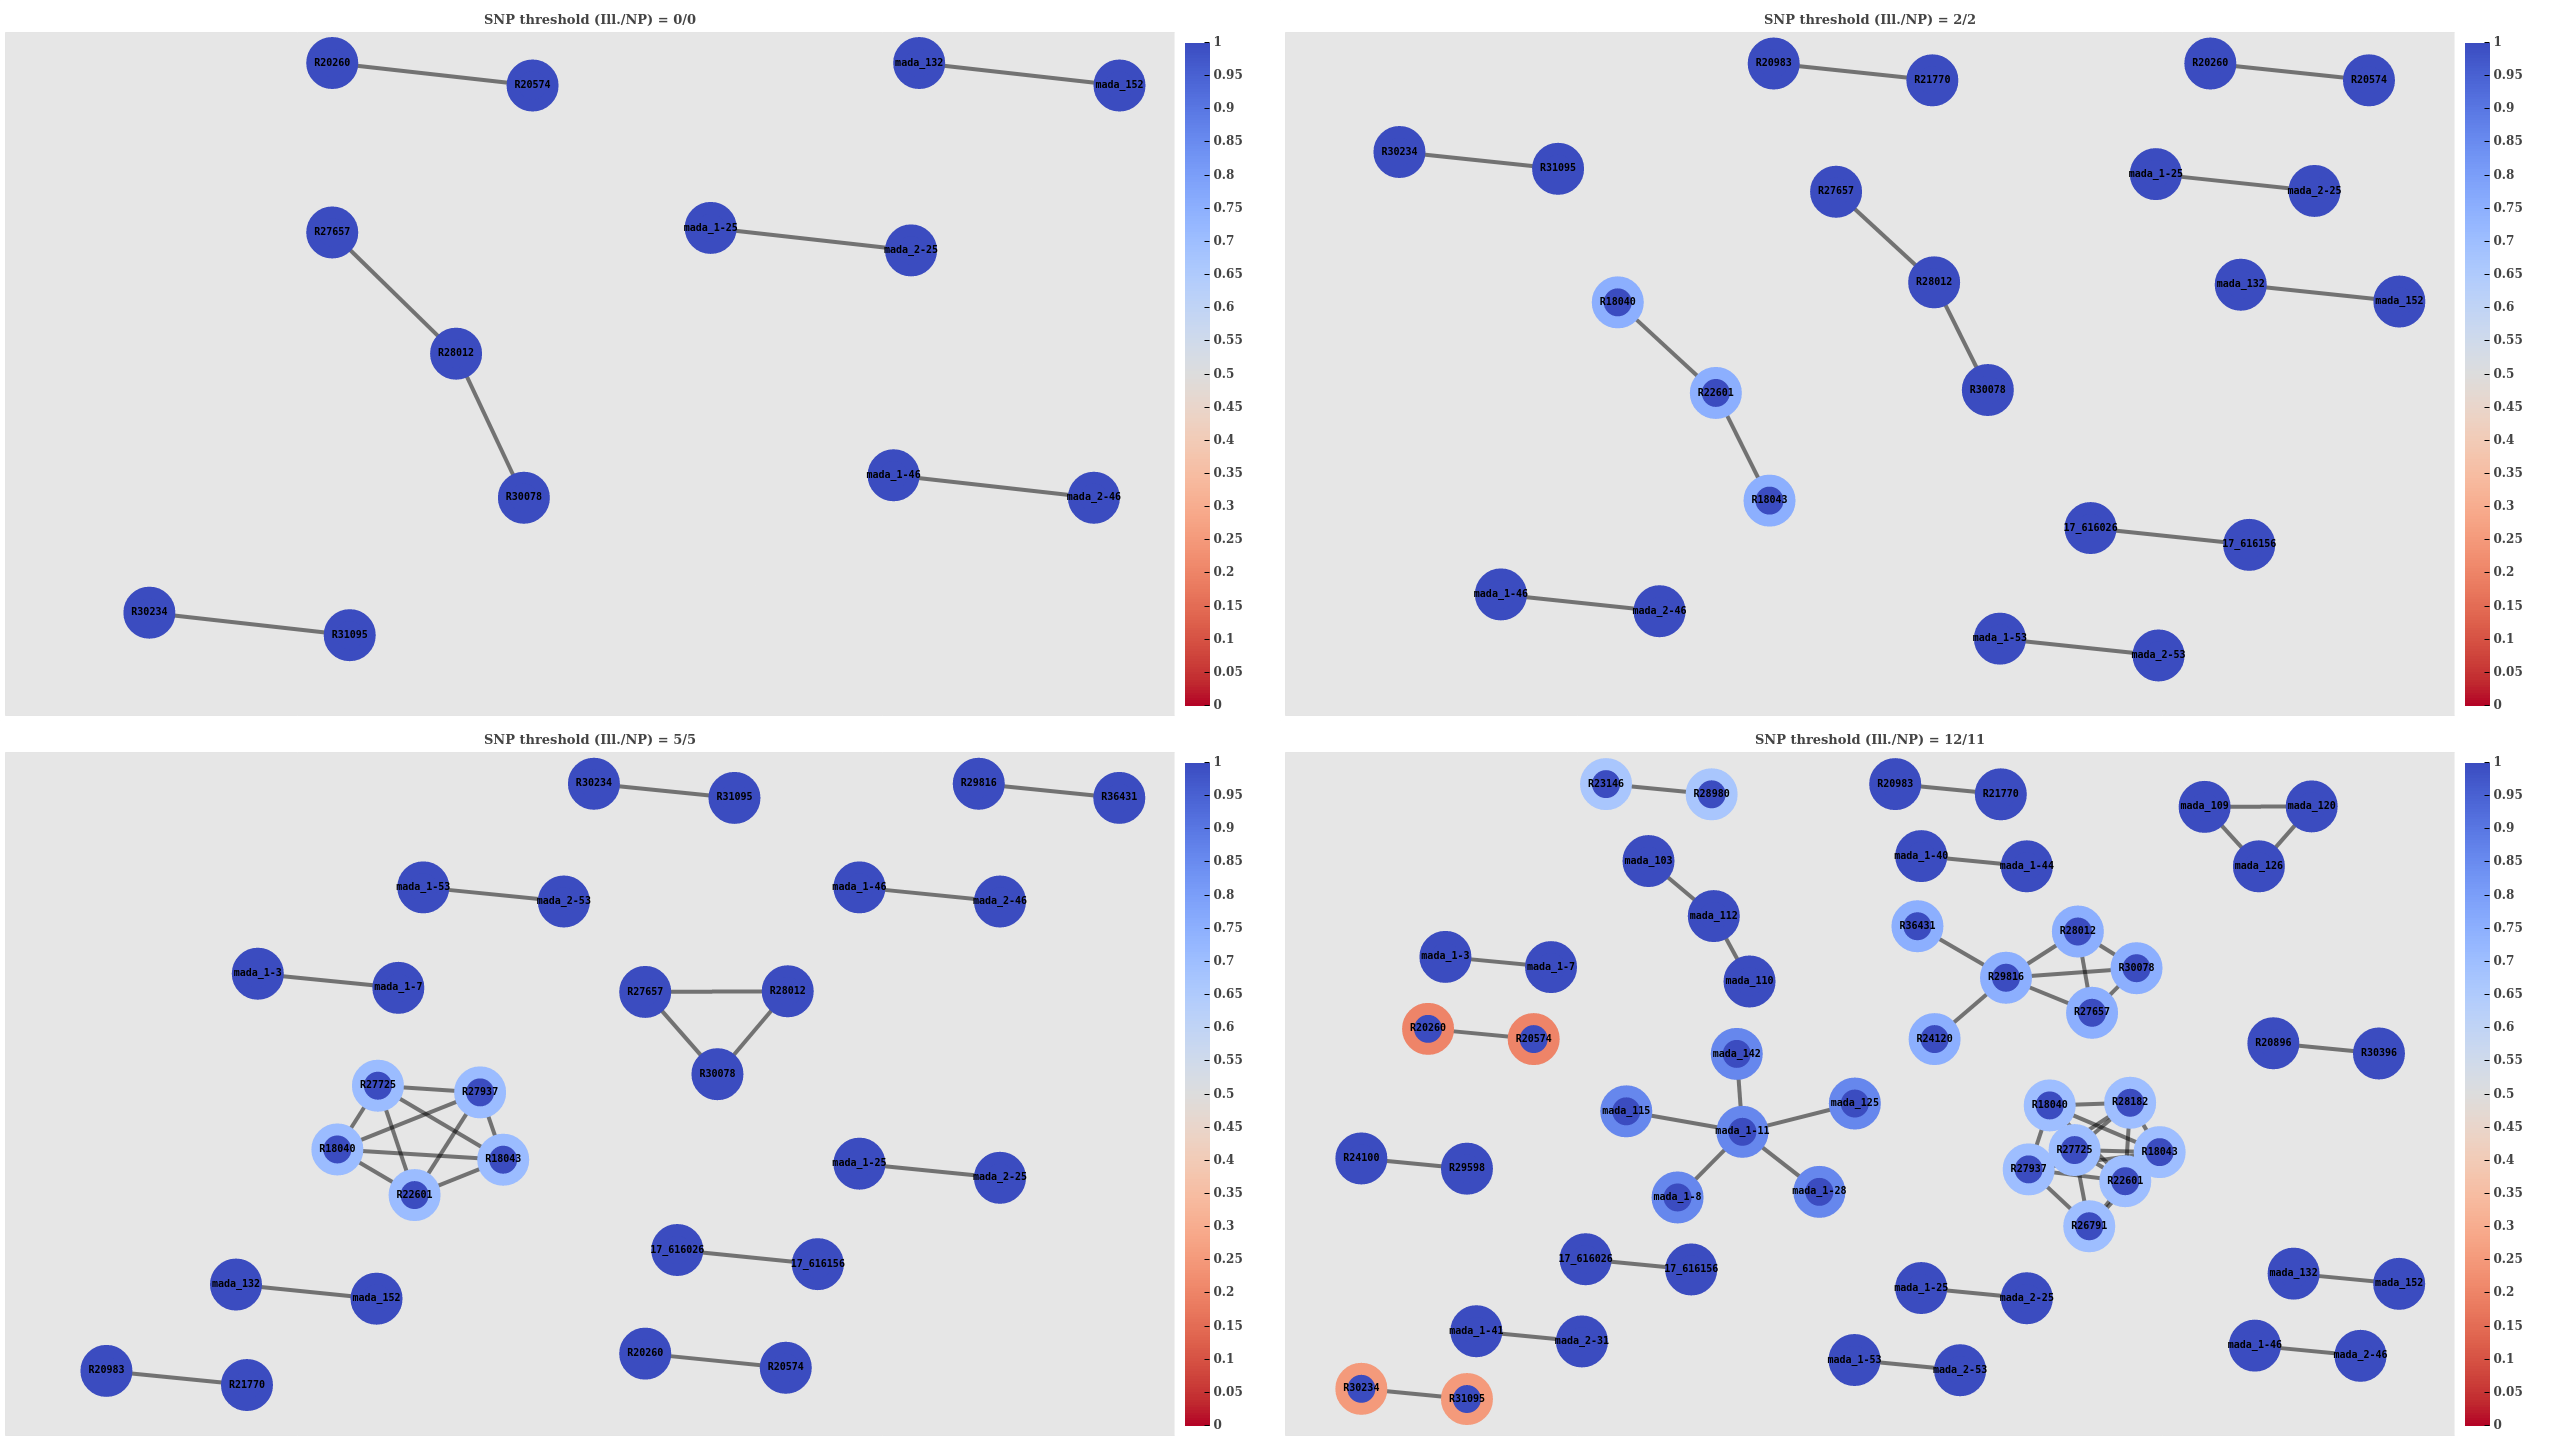
\includegraphics[width=0.70\columnwidth]{Chapter2/Figs/bcftools_clusters.png}
\caption{{Agreement of Illumina and Nanopore transmission clustering at SNP
thresholds 0 (top-left), 2 (top-right), 5 (bottom-left). The title of
each subplot indicates the Illumina (Ill.) and Nanopore (NP) threshold
used when clustering. Samples (nodes) are connected when the SNP
distance between them is less than or equal to the relevant threshold.
The inner and outer colours for each node indicates the SACR and SACP
values, respectively, for the cluster it is a part of. The
Illumina-based clustering is shown.
{\label{827243}}%
}}
\end{center}
\end{figure}

\subsection{Single-sample genome graph approach}

\subsection{Multi-samples genome graph approach}

%=========================================================================

\section{Constructing transmission clusters with mixed Illumina and \ont{} data}

Being able to deduce transmission clusters from a mixture of sequencing
modalities would allow greater integration across datasets from various
sources and prevent laboratories from being locked into any one
sequencing technology.

To this end, we investigate what the impact (if any) of combining
Illumina and Nanopore datasets has on SACR, SACP and XCR.

Firstly, we get a sense for how comparable the distances are likely to
be but looking at the ``self-distance'' for each sample - the distance
between a sample's Illumina and Nanopore data. This is shown in Figure
\todo{link}.

Next, we examine an array of Nanopore-to-Illumina ratios - 0.01, 0.05,
0.1, 0.25, 0.5, 0.75, and 0.9. When comparing two samples of the same
sequencing technology, we use the same SNP \emph{thresholds} as in
section \todo{link} and for mixed comparisons, we
use the same SNP threshold as Illumina.

For each ratio and SNP threshold combination we do the following 1000
times: 1) randomly assign samples to a technology in the relevant ratio,
2) calculate SACR, SACP, and XCR as per
section~\todo{link}. The simulations are visualised
in Figure~\todo{link} as violin plots in Python with
\texttt{matplotlib} and \texttt{seaborn} libraries.

Having established that Illumina-defined transmission clusters can be
confidently recreated with Nanopore data alone, the next logical
question is whether the same holds true when~\emph{mixing} Illumina and
Nanopore data. As the uptake of Nanopore sequencing increases it seems
inevitable there will be cases where comparisons between these
sequencing modalities is necessary. To address this question we simulate
varying degrees of Nanopore/Illumina mixtures and see how this impacts
clustering - using the above evaluation framework.

The first thing we look at is the mixed modality ``self-distance''. By
self-distance, we mean the distance between a sample's Illumina and
Nanopore data. As the sequencing data originates from the same source we
know the self-distance for any sample~\emph{should~}be 0. However, we
also know there are major technological differences between Illumina and
Nanopore, so it is wise to check just how similar they are.
Figure~\todo{link} shows a histogram of the
self-distance for all samples. We find a median of 0 and a mean of 1.
There is one major outlier, with a self-distance of 53. There is no
evidence of a sample mix-up for this particular isolate so we chose to
keep it in the analysis to account for the types of variation seen in
real data.

Next, we look at the pairwise SNP distance relationship, akin to that in
section~\todo{link}.
Figure~\todo{link} shows a similar relationship to
the single-technology correlation in Figure
\todo{link}. The difference here, however, is that
the y-axis represents the distance between one sample's Illumina data
and the other's Nanopore.~

We look at the transmission clusters for mixtures of Nanopore and
Illumina data using the same SNP thresholds used in
section~\todo{link}. For the comparison of different
modalities we use the same SNP thresholds as Illumina. The mixture
ratios we investigate are 0.01, 0.05, 0.1, 0.25, 0.5, 0.75, and 0.9.
That is, for a ratio of 0.25, we randomly allocate 25\% of the samples
to Nanopore and the remainder to Illumina. For each SNP threshold and
ratio, we calculate the XCR, SACR and SACP that the clustering produces
- using those ratio and threshold values. We repeat this process 1000
times for each threshold and ratio to simulate different mixtures of
sample-technology pairs. The simulation of so many different mixed pairs
is intended to provide insight into how robust clustering with mixtures
of sequencing dataset is likely to be. The results of these simulations
are shown in Figure~\todo{link}. We found that for
all SNP thresholds and ratios, the median SACR was 1.0. In other words,
regardless of the Nanopore/Illumina mixture ratio, for all thresholds we
used, no sample from the truth clusters is missed. The SACP values
decrease somewhat as the ratio leans more towards Nanopore data.
However, the lowest median SACP value was 0.845, which is also the SACP
value obtained for the Nanopore-only clustering in
section~\todo{link}. The XCR values tend to increase
slightly as more Nanopore samples are added. In the most extreme case,
0.057 was the highest XCR value in any simulation (SNP threshold 5).
Incidently, this is the same as the XCR obtained for the Nanopore-only
clustering of the same SNP threshold, which equates to 7 of the 122
non-clustered samples being clustered. However, regardless of the XCR,
no samples that should have been clustered were missed (on average).


\begin{figure}
\begin{center}
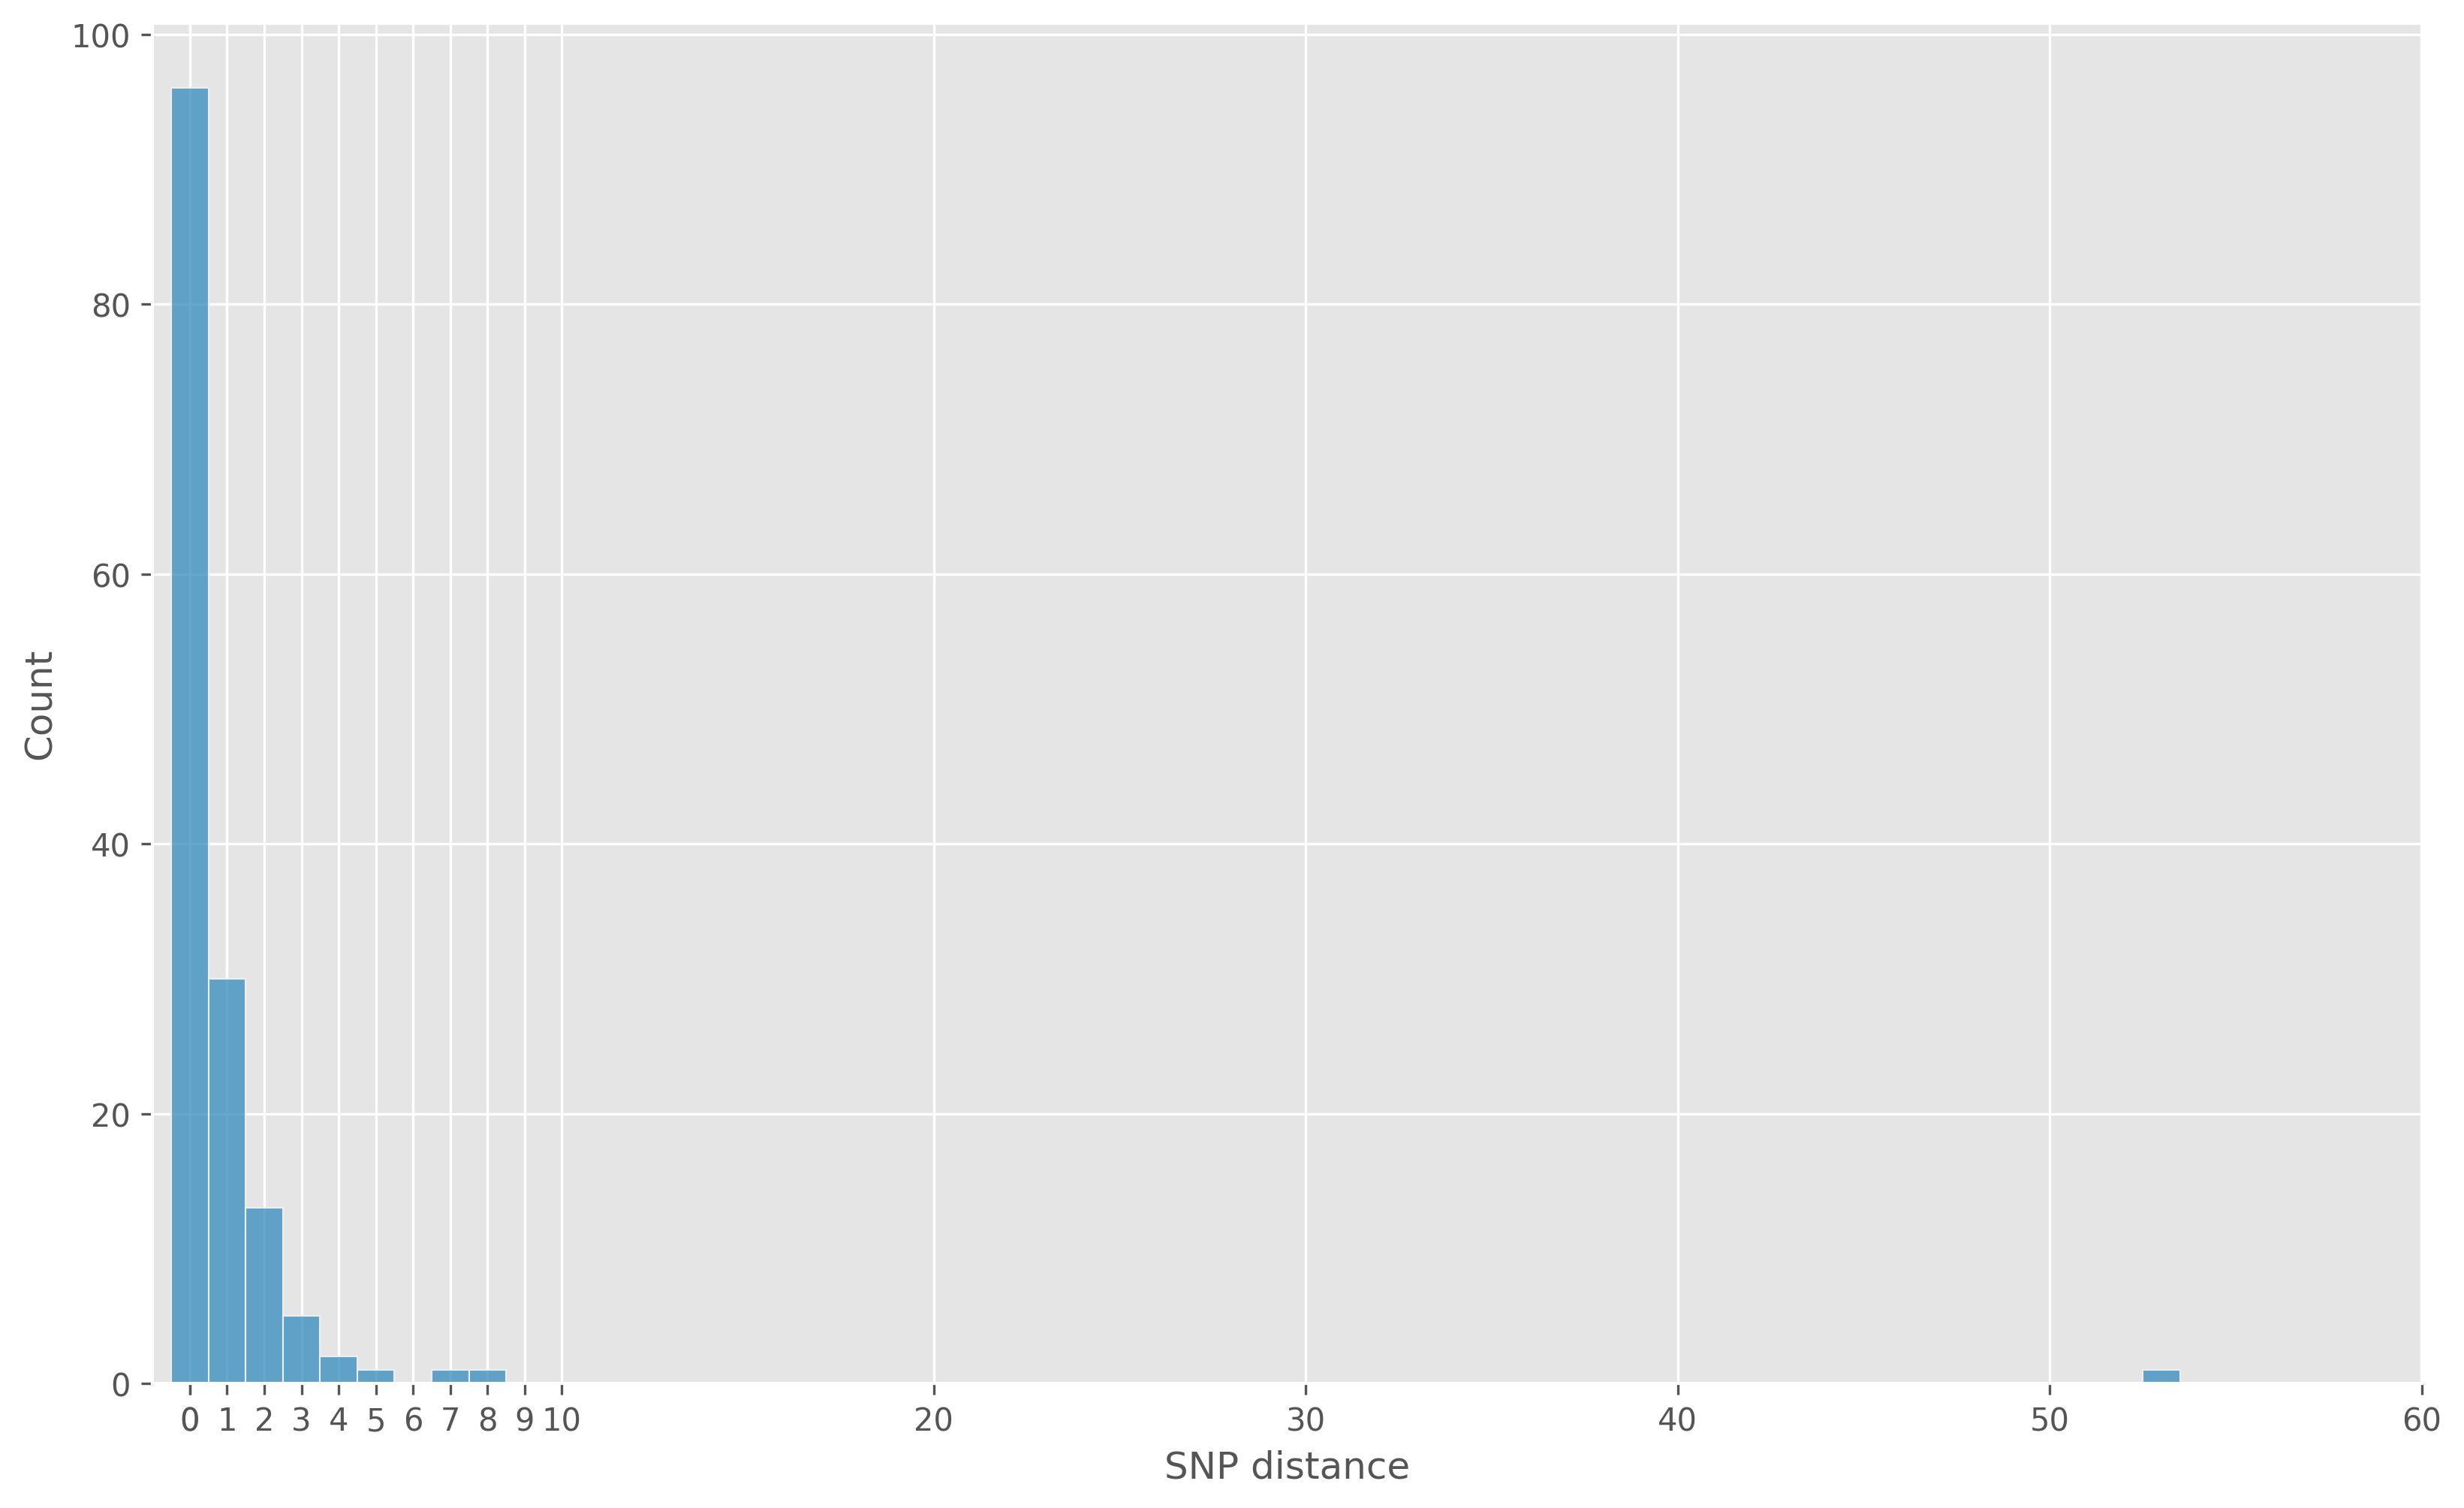
\includegraphics[width=0.70\columnwidth]{Chapter2/Figs/mixed_self_dist.png}
\caption{{Mixed modality "self-distance". This plot shows the SNP distance
(x-axis) between each sample's COMPASS (Illumina) and bcftools
(Nanopore) VCF calls.
{\label{166726}}%
}}
\end{center}
\end{figure}
\begin{figure}
\begin{center}
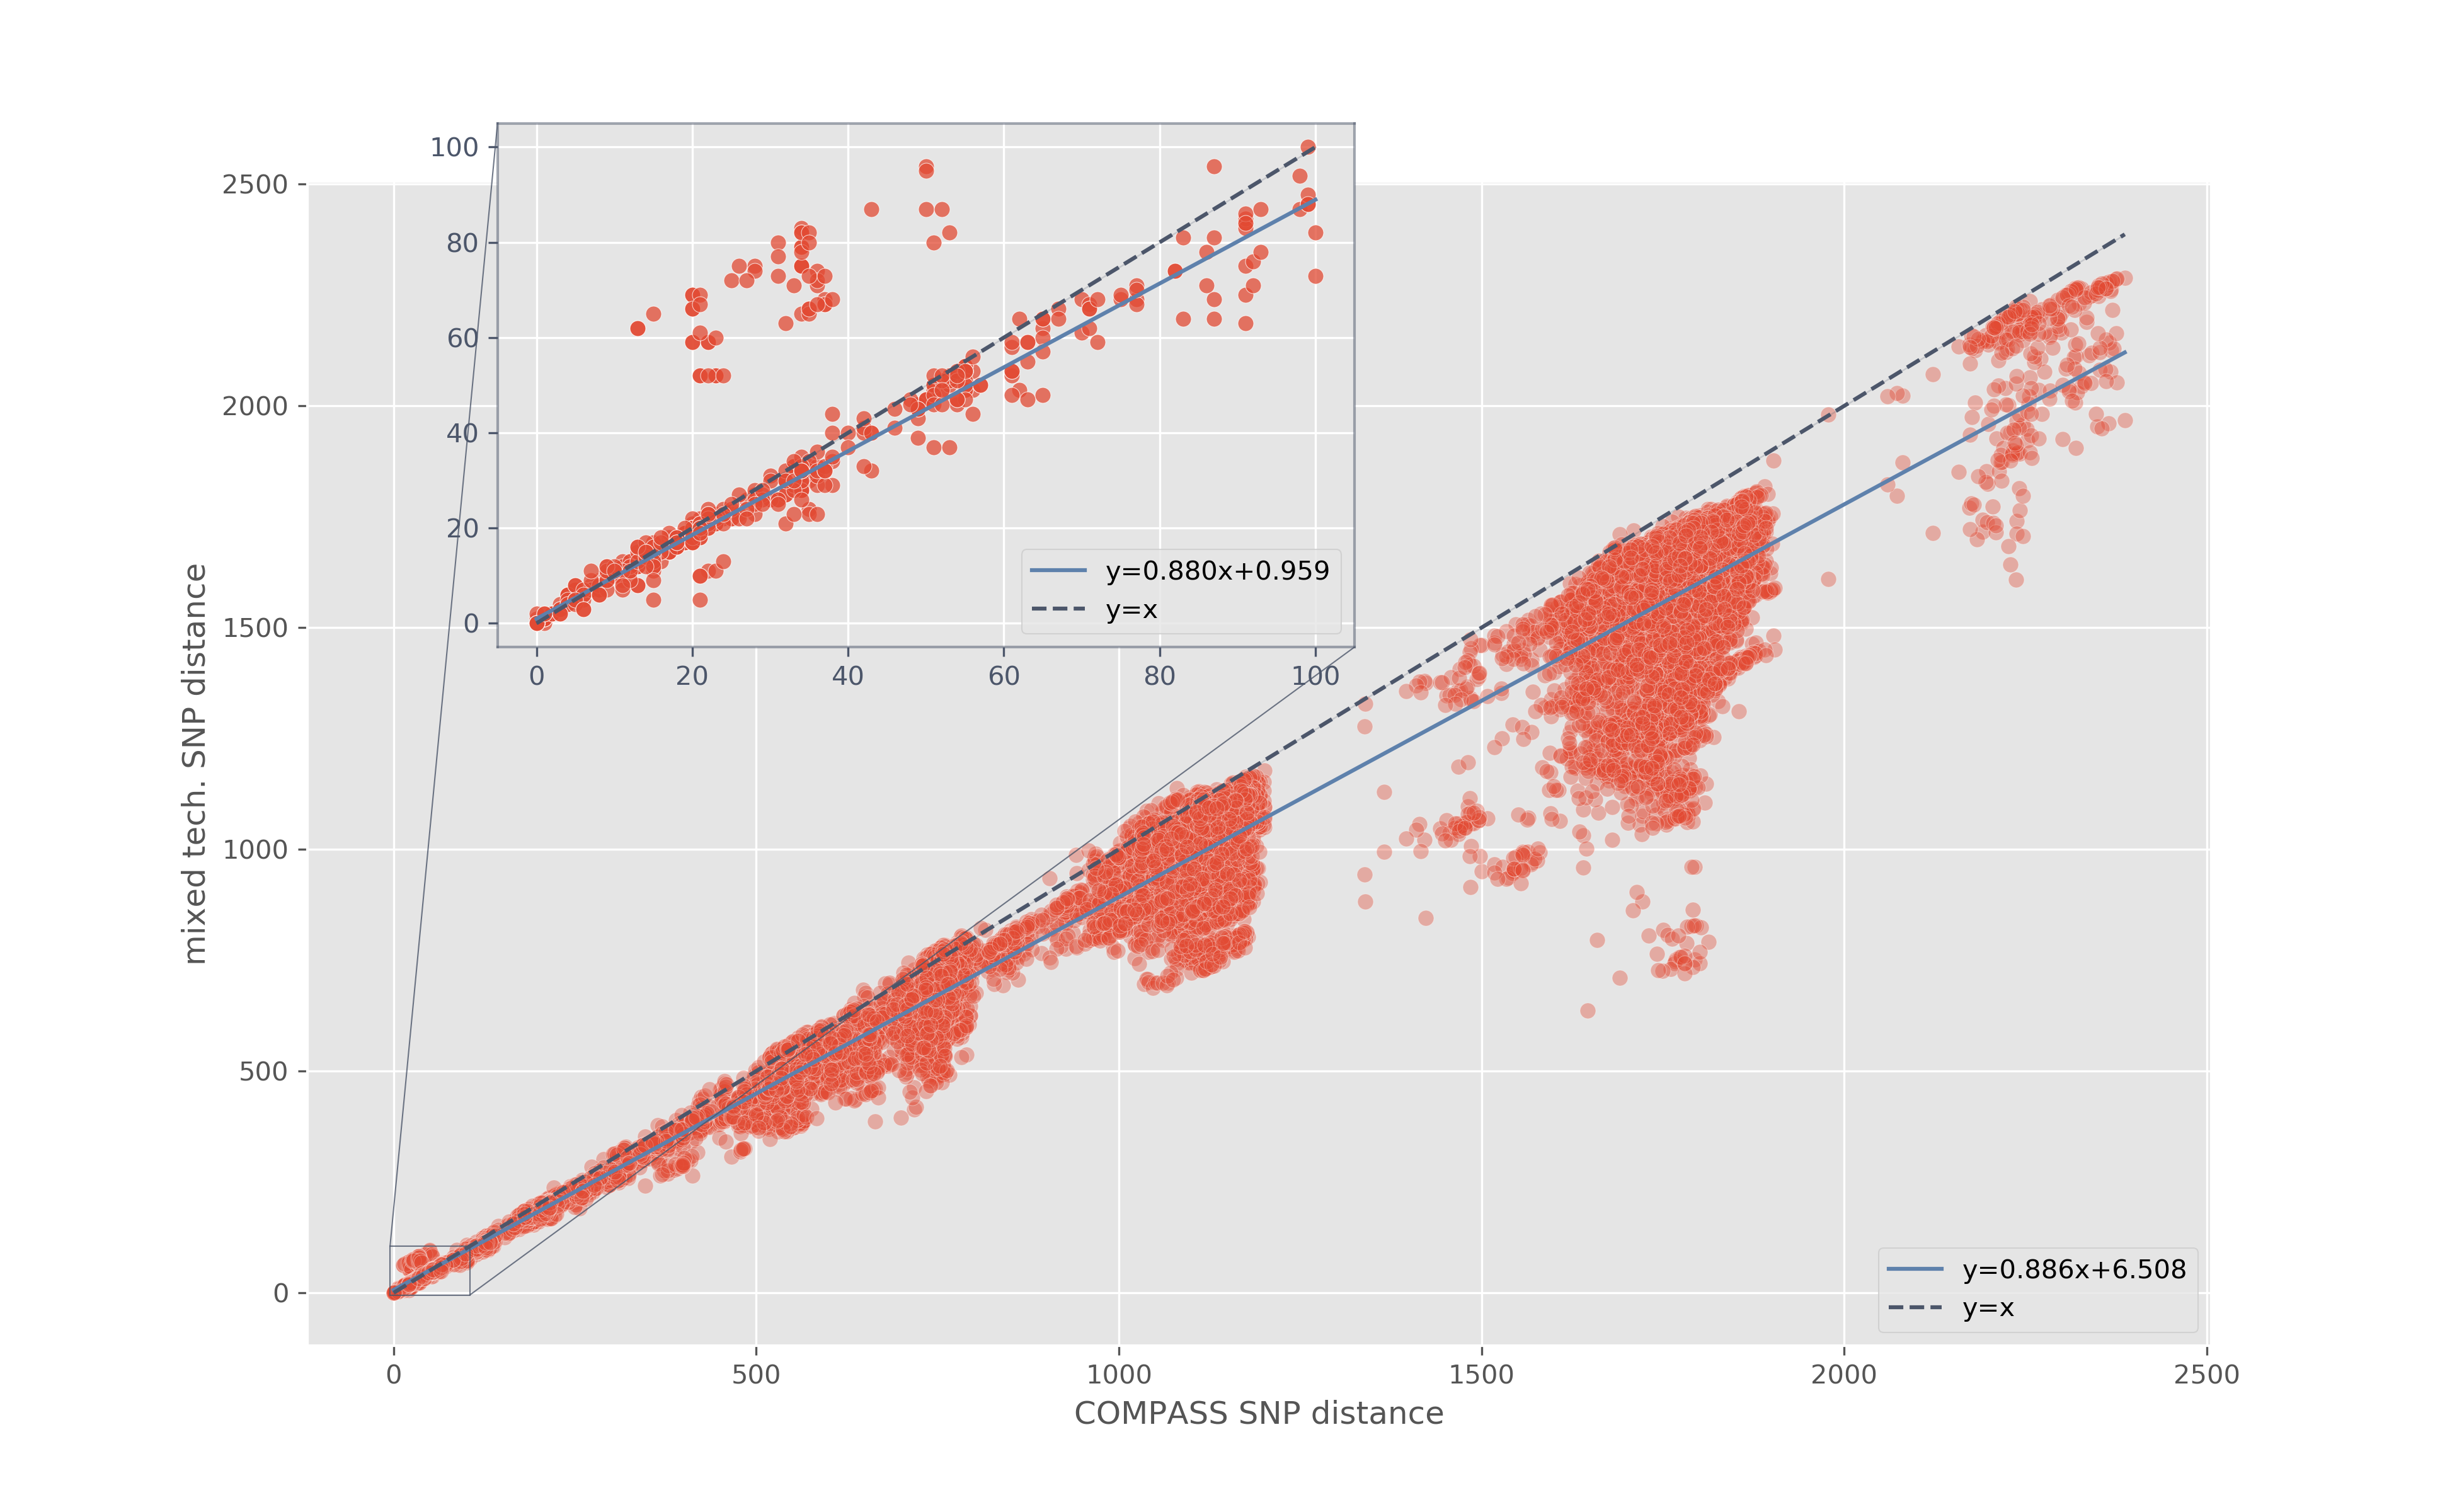
\includegraphics[width=0.70\columnwidth]{Chapter2/Figs/mixed-dotplot.png}
\caption{{The relationship of the distance between all pairs of samples based on
COMPASS VCF calls (X-axis) and mixed COMPASS-bcftools calls (Y-axis).
The black, dashed line indicates the relationship we would expect if the
distance between a pair of samples were the same for both approaches.
The blue line indicates the line of best fit based on fitting a robust
linear regression model to the data. The inset gives a closer look at
the relationship for all sample pairs where the COMPASS distance is less
than or equal to 100 SNPs. The legend indicates the linear equations for
the lines. Note: to prevent model skew, we do not include self-distance
pairs.
{\label{556408}}%
}}
\end{center}
\end{figure}
\begin{figure}
\begin{center}
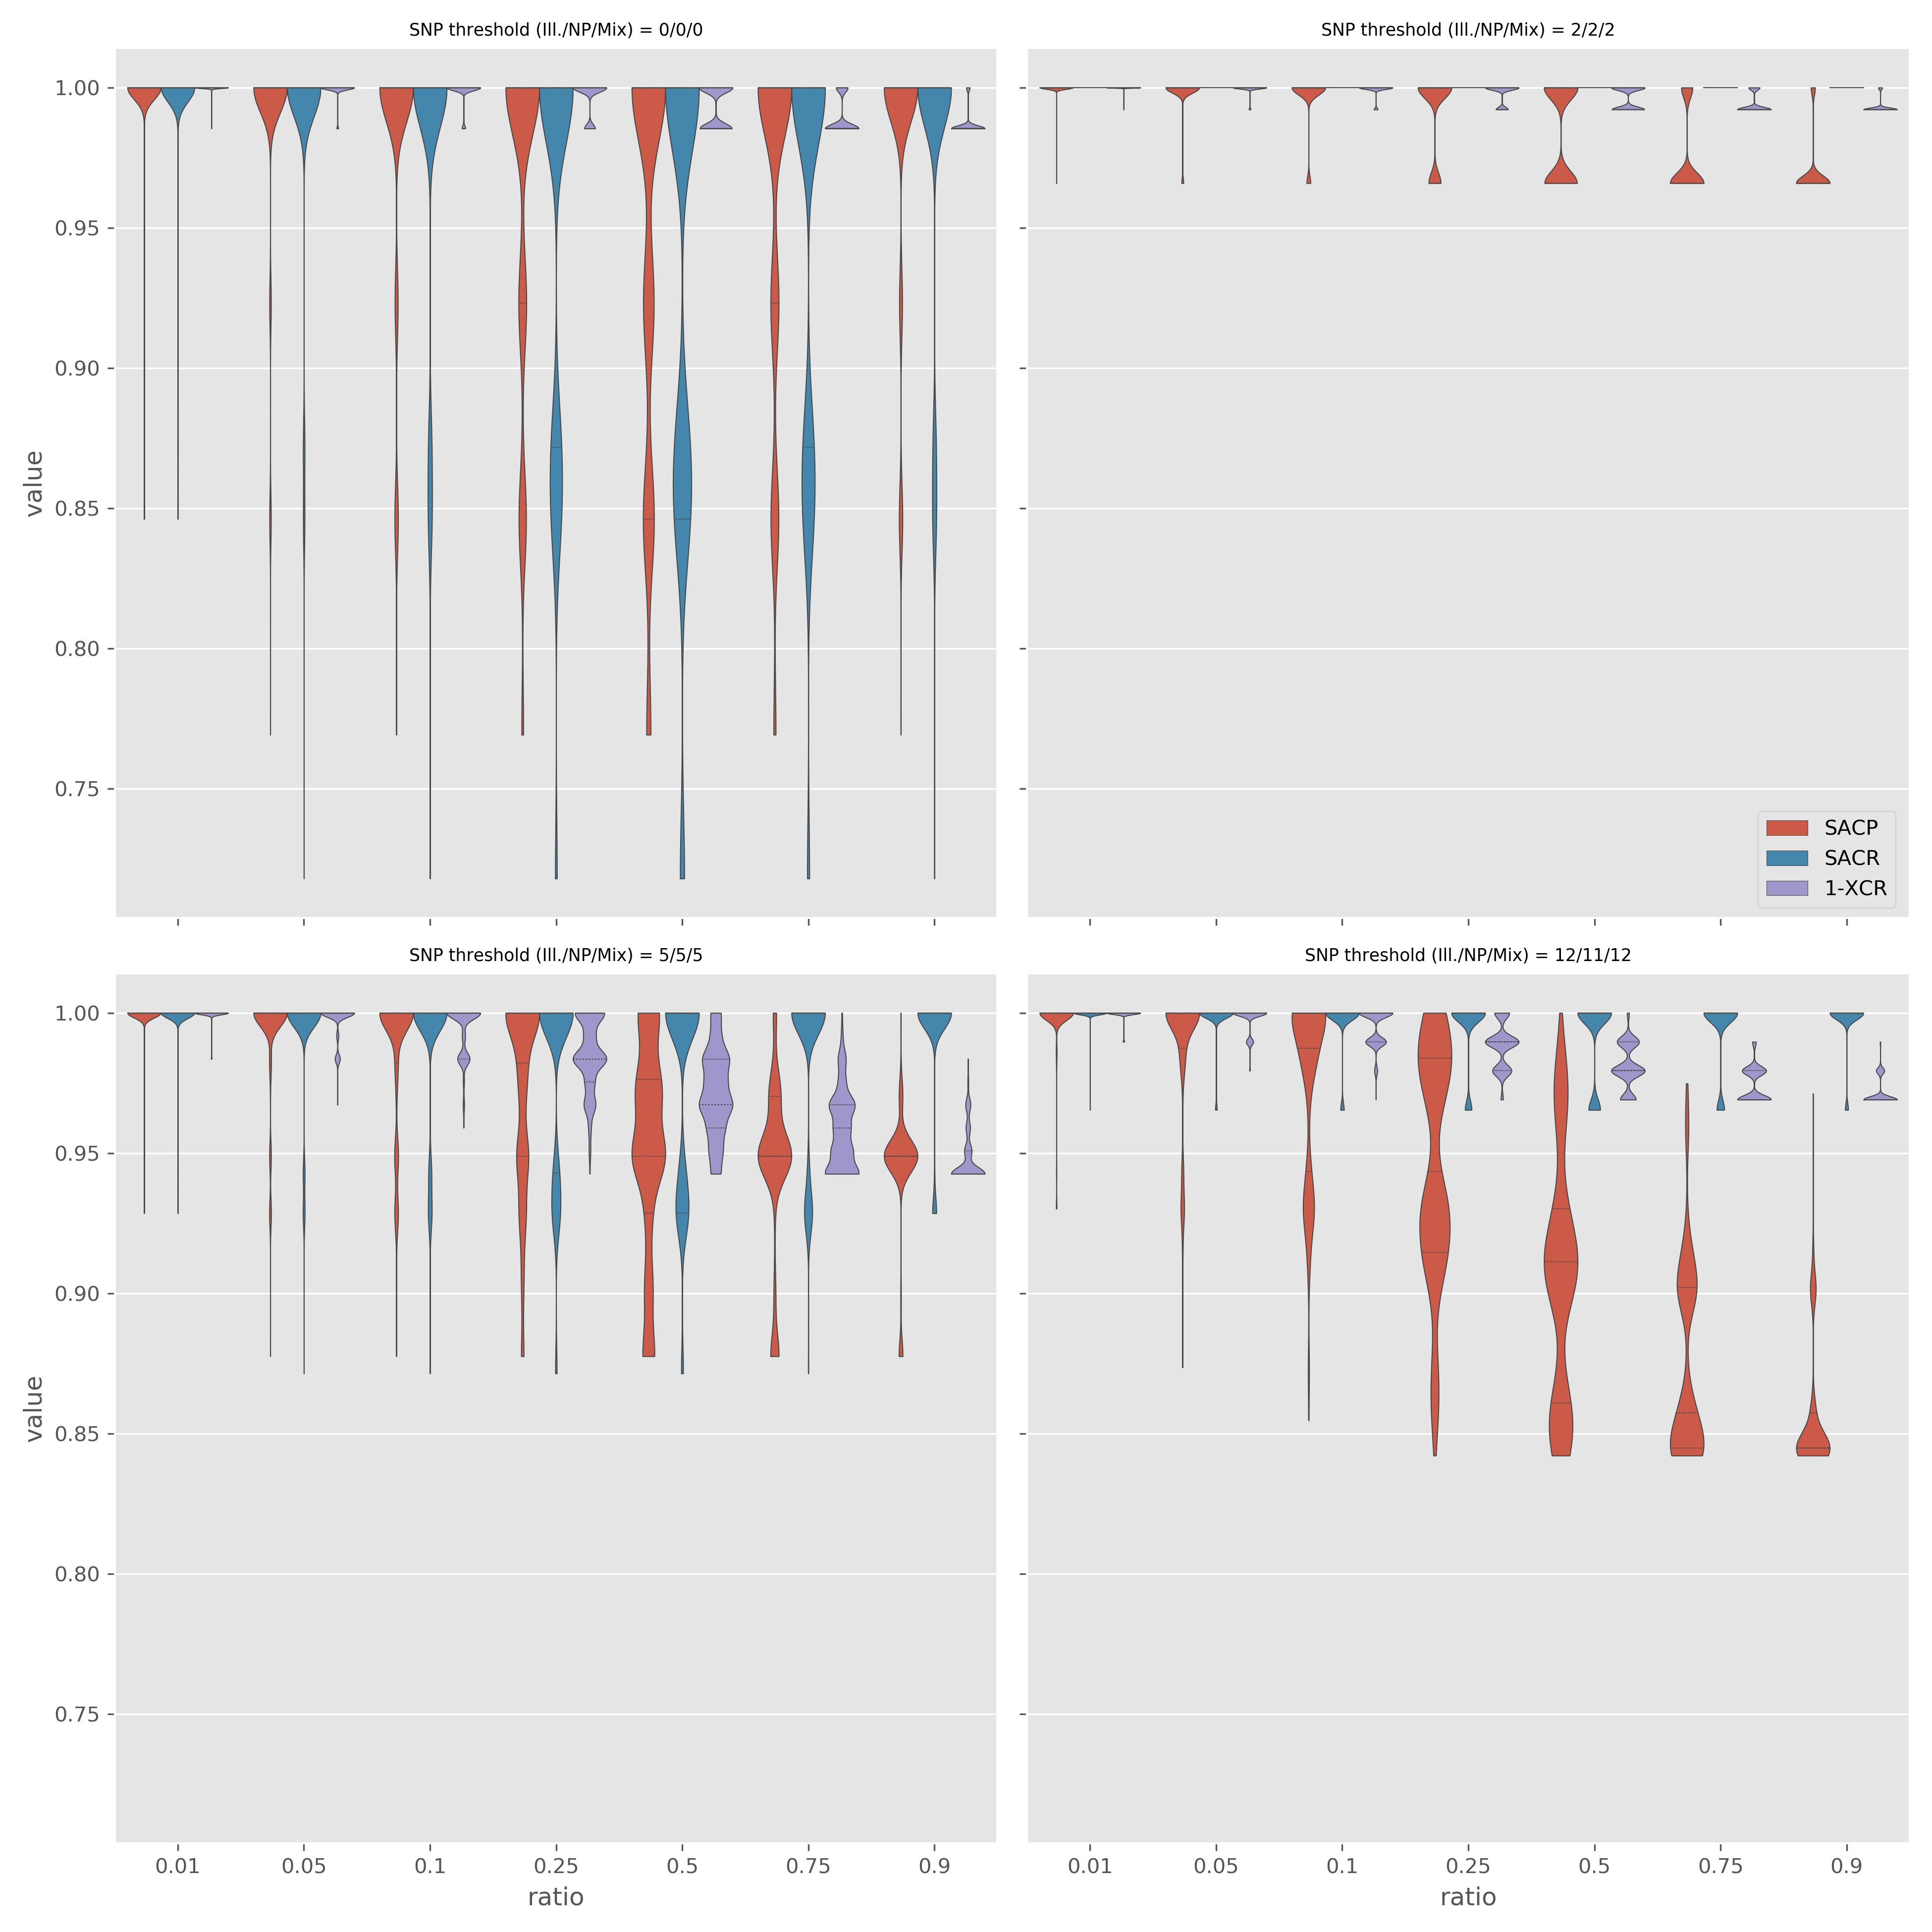
\includegraphics[width=0.70\columnwidth]{Chapter2/Figs/mixed_simulations.png}
\caption{{Simulating varying ratios (X-axis) of Nanopore/Illumina sample mixtures.
The different thresholds (subplots) indicate the cutoff for defining
samples as part of a cluster. The Y-axis depicts the Sample-Averaged
Cluster Precision and Recall (SACP/SACR) and Excess Clustering Rate
(XCR) distributions over all simulation runs (XCR is shown as (1-XCR)
for better axis-scaling). For each ratio/threshold combination we run
1000 simulations where the Nanopore and Illumina data is randomly split
into the relevant ratio and clusters are defined based on the relevant
threshold. The titles for each subplot indicate the SNP threshold use
when comparing Illumina (Ill.), Nanopore (NP), or mixed-technology
sample pairs.
{\label{571244}}%
}}
\end{center}
\end{figure}
%=========================================================================

\section{Discussion}

%=========================================================================

\section{Future work}


